\documentclass[a4j,dvipdfmx]{jsarticle}
\usepackage{amsmath,amssymb}
% \usepackage{fancybx}
\usepackage{fancyhdr}
\usepackage{ascmac}
\usepackage{siunitx}
\usepackage[dvips]{graphicx}

\renewcommand{\thesection}{\Roman{section}}
\renewcommand{\thesubsection}{\roman{subsection}}
% \renewcommand{\thesubsubsection}{\roman{subsubsection}}

\pagestyle{fancy}

\title{積分 解き方集}
\author{$\sum$理学愛好会}
\date{}

\begin{document}
\maketitle
\section{はじめに}
積分の計算は、難しい。微分は式変形をしなくても、公式を適応するだけで解くことができるが、積分はそうはいかない。
自分の計算しやすいように変形する必要があるのだ。うまく公式で扱える範囲に変形するにはある程度知識が必要だ。
だが、それ以上に経験がものをいう。そこで、今回は積分の計算力をつけるため、様々なパターンの積分を解いてもらう。
ある程度進めていくと、どういう式のときにどういう変形をすればいいかが見えてくるようになる。ぜひその``コツ''を
つかんでほしい。\\

この資料の構成としては、まず始めに積分の感覚をつかむための``基礎の基礎''の問題を載せている。とりあえずそこから取り組んで
いったん体をならすことをお勧めする。つぎに``基礎''の問題として、有理関数の積分や置換積分・部分積分の簡単な計算問題を載せている。
そのあとは、応用問題として少し難しい積分を載せている。積分問題をパターンで分類して、それぞれの解き方も解説していく。\\

また今回は、実際にこれまでの資料で扱わなかった特殊な積分を併せて紹介していく。それらも同時に覚えていくことで
自分の道具が増えていくことを実感してほしい。


\newpage
\tableofcontents
\clearpage

\part{不定積分}
\section{不定積分の基礎の基礎}
ここでは、置換積分や部分積分を用いないで、単純な変形だけで解ける問題を扱う。基本がわかっていないひとはここから読むべきである。
\subsection{多項式の積分}
ここでは多項式の積分について扱う。先に言葉の復習から行う。多項式とは、
\begin{equation*}
    P(x)=a_0 x^n +a_1 x^{n-1} +\cdots+a_{n-1}x+a_n\quad(\text{$a_0,\cdots,a_n$は定数 $n>1$})
\end{equation*}
となるような$P(x)$のことである。また$P(x)$を$x$についての多項式ともいう。

さて、多項式の積分であるが、これらは$x$のべき乗の和であるため個別に積分できて、
\begin{equation*}
    \int P(x)dx=\int a_0x^ndx +\int a_1 x^{n-1}dx+\cdots+\int a_{n-1}xdx+\int a_ndx
\end{equation*}
となる。それぞれの項の積分は簡単に求められる。
\subsubsection{例題}
\begin{equation*}
    \int (4x^3+3x^2+2x)dx
\end{equation*}
を求めよ。
\subsubsection*{解答}
個別に積分すると、
\begin{equation*}
    \int (4x^3+3x^2+2x)dx=\int 4x^3dx+\int 3x^2dx+\int 2xdx=x^4+x^3+x^2+C
\end{equation*}
となる。最後の積分定数を忘れないように。

\subsubsection{例題}
\begin{equation*}
    \int (x^2+1)^2dx
\end{equation*}
を求めよ。
\subsubsection*{解答}
展開すれば、個別に積分できるので、
\begin{equation*}
    \int (x^2+1)^2dx=\int (x^4+2x^2+1)dx=\int x^4dx+\int 2x^2dx+\int dx=\frac{x^5}{5}+\frac{2}{3}x^3+x+C
\end{equation*}
このように、積の形であっても\underbar{展開して和に直すことで}、個別に積分できる。個別に撃破すれば恐れることはない。
\subsection{三角関数の積分}
次はみんな大好き三角関数の積分である。符号にさえ注意すればそこまで恐れることはない。ただ、
三角関数の公式を把握していないと、$\sin x,\cos x$はできるかもしれないが、これが$\sin^2 x,\cos^2 x$となった
ときに計算できなくなってしまう。曖昧な公式があれば復習をするとよい。
\subsubsection{例題}
次の積分を求めよ。
\begin{equation*}
    \int (\sin x+\cos x) dx
\end{equation*}
\subsubsection*{解答}
個別に積分してしまえば一発である。
\begin{equation*}
    \int(\sin x+\cos x)dx=\int \sin xdx+\int \cos xdx=-\cos x+\sin x+C
\end{equation*}
\subsubsection{例題}
次の積分を求めよ。
\begin{equation*}
    (1)\int \sin^2 \frac{x}{2}dx\quad (2)\cos^2 \frac{x}{2}dx 
\end{equation*}
\subsubsection*{解答}
これまでのようにすでに和の形になっていないので最初は戸惑いやすい。半角の公式を使ってしまえば和の形に変形できる。
\begin{align*}
    &(1)\int \sin^2 \frac{x}{2}dx=\int\frac{1-\cos x}{2}dx=\frac{1}{2}(\int dx-\int \cos xdx)=\frac{1}{2}(x-\sin x)+C\\
    &(2)\int \cos^2 \frac{x}{2}dx=\int\frac{1+\cos x}{2}dx=\frac{1}{2}(\int dx+\int \cos xdx)=\frac{1}{2}(x+\sin x)+C 
\end{align*}
この変形は実は結構よく使う。絶対に覚えておくべき変形である。
\newpage
\subsection{指数関数の積分}
ここでは指数関数を扱う。微分しても積分しても形が変わらない$e^x$という特殊な関数をメインで扱う。
\subsubsection{例題}
次の積分を求めよ。
\begin{equation*}
    (1)\int 2^x dx\quad(2)\int e^{x+1}dx
\end{equation*}
\subsubsection*{解答}
(1)公式をそのまま適応して、
\begin{equation*}
    \int 2^x dx=\frac{2^x}{\log 2}+C
\end{equation*}

(2)指数法則$a^b\cdot a^c=a^{b+c}$をもちいて、
\begin{equation*}
    \int e^{x+1}dx=e\int e^xdx=e^{x+1}+C
\end{equation*}
(2)の問題は普通は置換積分を使うが、指数法則を用いても解くことができるということを知ってほしい。\\
\hrulefill
\subsection{演習問題}
以下の積分を求めよ。\\
(1)$\displaystyle\int \sqrt{x}(x^2+1)dx$
\hspace*{20mm}
(2)$\displaystyle\int\sin(x-\frac{\pi}{2})dx$
\hspace*{20mm}
(3)$\displaystyle\int 2\cos xdx$
\\\\
(4)$\displaystyle \int (\cos^2\frac{x}{2}+\sin^2\frac{x}{2})dx$
\hspace*{12mm}
(5)$\displaystyle\int2^{\log x}dx$

\newpage

\section{不定積分の基礎}
ここでは、置換積分・部分積分、有理関数の積分を主に扱う。置換積分、部分積分をなくしては
積分の問題は解くことができない(たまに微分から逆算することもできるが)。有理関数も有理関数の不定積分
が必ず求められることから非常に重要になってくる。この重要性については応用問題の際に語るとして、とりあえず
簡単な問題から取り組んでいこう。
\subsection{置換積分の基礎}
始めに置換積分について扱う。もっとも汎用性が高い変形方法ではないだろうか。一応、置換積分の公式を書いておく。
\begin{equation*}
    \int f(x)dx = \int f(\phi(t))\phi'(t)dt
\end{equation*}
\subsubsection{例題}
次の不定積分を求めよ。
\begin{equation*}
    (1)\int (2x+1)^3 dx \quad (2)\int\tan x dx \quad (3)\int\cos^2 xdx
\end{equation*}
\subsubsection*{解答}
(1)展開して各項ごとに積分することもできるが、置換積分を使ったほうが圧倒的に早い。
$t=2x+1$と置くと、$dt=2dx$より、
\begin{equation*}
    \int \frac{1}{2}t^3dt=\frac{1}{8}t^4+C =\frac{1}{8}(2x+1)^4+C
\end{equation*}
最後に$x$の式に戻すことを忘れないように。

(2)$\tan x=\sin x/\cos x$の公式と$(\cos x)'=-\sin x$を利用し、$t=\cos x$と置くと、
\begin{equation*}
    -\int \frac{(\cos x)'}{\cos x}dx=-\int \frac{1}{t}dt=-\log |t|+C=-\log|\cos x|+C
\end{equation*}

(3)半角の公式を使い、$t=2x$と置くことで、
\begin{equation*}
    \int \frac{1+\cos 2x}{2}dx=\frac{1}{2}(x+2\int \cos tdt)=\frac{1}{2}(x+2\sin 2x)+C
\end{equation*}
慣れてくると、(1)や(2)の問題程度ならわざわざ置換しなくても解くことができるようになる。

置換積分のポイントは、$t=f(x)$と置いたときに発生する$f'(x)$をどう処理するかである。例えば例題(2)では、
$t=\cos x$と置いているが、これは$dt=-\sin x dx$の$\sin x$がちょうど分子にあるからできることなのだ。
よって、うまく微分したらうまく重なるところを探す必要がある。
\subsubsection{例題}
$\displaystyle \int x\sin(x^2)dx$を求めよ。
\subsubsection*{解答}
$t=x^2$と置くと、$\frac{1}{2}dt=xdx$となり、式が簡単になる。
$\displaystyle \frac{1}{2}\int \sin tdt=-\frac{1}{2}\cos t+C=-\frac{1}{2}\cos (x^2)+C$
\newpage
\subsection{部分積分の基礎}
次は部分積分である。置換積分に比べたら使う機会は少ないかもしれないが、使えないと確実に困る。
例えば、今年の京大数学の第一問は部分積分で解く。まず置換積分同様、公式を載せる。
\begin{equation*}
    \int f(x)g'(x)dx=f(x)g(x)-\int f'(x)g(x)dx
\end{equation*}
式だけでは感覚はつかみにくいだろうから、試しに例題を解いてみよう。
\subsubsection{例題}
次の不定積分を求めよ。
\begin{equation*}
    (1)\int x\sin xdx\quad (2)\int xe^x dx \quad (3)\int x\log x dx
\end{equation*}
\subsubsection*{解答}
(1)$f(x)=x,g'(x)=\sin x$と置くと、
\begin{equation*}
    \int x\sin x dx=-x\cos x+\int \cos xdx=-x\cos x+\sin x+C 
\end{equation*}

(2)前問と同様に$f(x)=x,g'(x)=e^x$と置くと、
\begin{equation*}
    \int xe^x dx=xe^x-\int e^xdx=xe^x-e^x+C=(x-1)e^x +C
\end{equation*}

(3)今度は$f(x)=\log x,g'(x)=x$と置くと、
\begin{equation*}
    \int x\log xdx=\frac{1}{2}x^2\log x-\int \frac{1}{2}xdx=\frac{1}{2}x^2\log x-\frac{1}{4}x^2+C
\end{equation*}

例題を見ればわかるように、$xf'(x)$の積分は、$x$を微分することで$f(x)$の積分に変形できる。ただ、
$f(x)$の積分が余りにも複雑な場合には、この変形は使わないほうが良いかもしれない。(3)は、$(\log x)'=\frac{1}{x}$
に気づけば、$x$の積分に変形できる。このような積分は後ほど詳しく学ぶ。
\subsubsection{例題}
次の不定積分を求めよ。
\begin{equation*}
    \int e^x \cos xdx
\end{equation*}
\subsubsection*{解答}

とりあえず、この不定積分を$I$と置いて計算する。二回部分積分を行うと、
\begin{equation*}
    I=\int e^x \cos xdx=e^x\cos x + \int e^x \sin xdx=e^x\cos x+e^x \sin x-I 
\end{equation*}
よって、
\begin{equation*}
    I=\frac{e^x}{2}(\cos x+\sin x)+C
\end{equation*}
このように部分積分を行い、右辺に求めたい積分をつくることで積分を計算することもできる。
\newpage
\subsection{有理関数の積分の基礎}
最後に有理関数の積分についてである。先に有理関数の定義を述べておく。$f(x),g(x)$をそれぞれ多項式とすると、
有理関数$F(x)$は次にようになる。
\begin{equation*}
    F(x)=\frac{f(x)}{g(x)}
\end{equation*}
一般に、\underbar{有理関数の積分は常に求められる}。下線部の性質はとても重要で、これを用いれば、被積分関数を$x$に関する
有理関数に帰着することが出来れば、その積分は必ず求められることになる。
そのため、有理関数の積分を求める練習はしておいたほうが良いだろう。
\subsubsection{例題}
次の不定積分を求めよ。
\begin{equation*}
    (1)\int \frac{x+5}{x-2}dx\quad(2)\int \frac{x^3+2}{x^2+1}dx\quad(3)\int \frac{dx}{x^2-9}
\end{equation*}
\subsubsection*{解答}
(1)$\displaystyle \frac{x+5}{x-2}=1+\frac{7}{x-2}$という風に変形を施せば、
\begin{equation*}
    \int 1+\frac{7}{x-2}dx=x+7\int \frac{dx}{x-2}=x+7\log|x-2|+C
\end{equation*}
(2)商とあまりの和の形になおしてあげると、
\begin{equation*}
    \int \frac{x^3+1}{x^2+1}dx=\int x+\frac{2-x}{x^2+1}dx=\frac{1}{2}x^2+2\arctan x - \log(x^2+1)+C
\end{equation*}
(3)そのままでは積分できないので、もちろん変形しなければならない。
\begin{equation*}
    \int \frac{dx}{x^2-9}=\int\frac{dx}{(x-3)(x+3)}=\frac{1}{6}\left(\int \frac{dx}{x-3}-\int\frac{dx}{x+3}\right)
    =\frac{1}{6}\left(\log |x-3|-\log|x+3|\right)+C=\frac{1}{6}\log \left|\frac{x-3}{x+3}\right|+C
\end{equation*}
このように部分分数分解を行うことで計算できる。
\subsubsection{例題}
次の不定積分を求めよ。
\begin{equation*}
    \int \frac{2}{x^2-2x-3}dx
\end{equation*}
\subsubsection*{解答}
部分分数分解によって、$\displaystyle\frac{2}{x^2-2x-3}=\frac{2}{(x-3)(x+1)}=\frac{1}{2}\left(\frac{1}{x-3}-\frac{1}{x+1}\right)$
と変形できるので、
\begin{equation*}
    \int\frac{2}{x^2-2x-3}dx=\int \frac{1}{2}\left(\frac{1}{x-3}-\frac{1}{x+1}\right)dx=\frac{1}{2}\log\left|\frac{x-3}{x+1}\right|+C
\end{equation*}
\newpage
\subsection{演習問題}
次の不定積分を求めよ。

$(1)\displaystyle\int (x+2)^{100}dx$
\hspace{20mm}
$(2)\displaystyle\int \sin^3 x\cos xdx$
\hspace{20mm}
$(3)\displaystyle\int x\cos xdx$\\

$(4)\displaystyle\int \log xdx$
\hspace{27mm}
$(5)\displaystyle\int x\sin(x^2)dx$
\hspace{24mm}
$(6)\displaystyle\int \sqrt{x}\log(x^2)dx$\\

※(6)の問題は、今年の京大数学の問題を一部変えて修正している。\\
\hrulefill
\subsection{$\blacksquare$Coffee Break: $\log |x|$ の絶対値記号}
\begin{screen}
    $\displaystyle\frac{1}{x+a}$の積分が何かと聞かれたら、もちろん$\log|x+a|$と答えるだろう。
    では、$\displaystyle\frac{2x}{x^2+1}$の場合ならどうか?$t=x^2+1$と置換すれば求まるがその答えを
    $\log|x^2+1|$と書いてしまっていないだろうか?$x^2+1$は最小値が$1$の関数である。すなわち、
    常に正なわけである。つまり、$|x^2+1|$は$(x^2+1)$と書くべきなのだ。そもそも、絶対値記号がつくのは、
    真数条件を満たすようにするためである。常に満たしている$x^2+1$に絶対値をつけるのは、おかしいのである。

    ちなみに、複素数まで数を拡張すれば、真数に負の値が入っても問題ない。(例:$\log(-1)=\pi i$)
\end{screen}
\newpage
\section{置換積分}
ここでは置換積分を中心に扱っていく。様々な置換の方法、テクニックを紹介する。
\subsection{$\sqrt{ax^2+bx+c}$の積分}
ひとまず、無理関数の積分から解いてみよう。無理関数の積分といっても様々な形があるが、今回は$\sqrt{ax^2+bx+c}$
に絞って扱っていく。
\subsubsection{$\sqrt{a^2-x^2}$の積分}
まず、$\sqrt{a^2-x^2}$の積分から解く。こういうタイプの積分は、まず根号を外すことを考える。
ここで三角関数の公式$\cos^2 x=1-\sin^2 x$を思い出してみよう。右辺がなんとなく$a^2-x^2$に似ている。
頑張って、$1-\sin^2 x$の形に持ってくれば、$\sqrt{\cos^2 x}=\cos x$となり根号が外れて計算しやすくなる。

よって、$x=a\sin \theta$の置換を行えばよいことがわかる。$dx=a\cos \theta d\theta$であるため、
\begin{equation*}
    \int \sqrt{a^2-x^2}dx=\int \sqrt{a^2-a^2\sin^2\theta}\cdot a\cos\theta d\theta
    =a^2\int \cos^2\theta d\theta=\frac{1}{2}(\theta+\frac{1}{2}\sin(2\theta))+C
\end{equation*}
ここで、$\theta =\arcsin(\frac{x}{a})$より、
\begin{equation*}
    \frac{1}{2}(\theta+\frac{1}{2}\sin(2\theta))+C=\frac{1}{2}(\arcsin(\frac{x}{a})+\frac{x}{a^2}\sqrt{a^2-x^2})+C
\end{equation*}
最後の式変形は$\sin(2\theta)=2\sin\theta\cos\theta$を用いた。

\subsubsection{$\sqrt{x^2+a^2}$の積分}
お次は、$\sqrt{x^2+a^2}$の積分である。これには複数のやり方がある。まず最初に思いつくのが$x=a\tan \theta$の置換だろう。
先ほどの$\sqrt{a^2-x^2}$の積分と同様に、三角関数を用いて根号を外せばいい。ただ、この方法は計算量がほかの方法に比べて多くなってしまう。\\

そこで、$x=a\sinh \theta$と置換することで、計算量を抑えることができる。$\sinh x$を知らない人がいるかもしれないので説明しておくと、
これは双曲線関数と呼ばれ、$\displaystyle \sinh x=\frac{e^x-e^{-x}}{2}$である。読み方は、「ハイパボリックサイン」である。$sin x$と
似た形をしているのは、$\sin x$にとても性質が似通っているからである。もちろん$\cosh x$もある。こちらは$\displaystyle \cosh x=\frac{e^x+e^{-x}}{2}$
となる。ちょっと考えればわかるように$\cosh^2 x=1+\sinh^2 x$である。この性質を利用して、
\begin{equation*}
    \sqrt{1+\sinh^2 x}=\cosh x
\end{equation*}
となれば、根号を外すことができるのだ!\\

とりあえず、今言った2つの方法でそれぞれ積分してみる。
\newpage
まず、$x=a\tan\theta$と置換してみる。
\begin{align*}
    I&=\int \sqrt{x^2+a^2}dx=a^2\int \frac{1}{\cos \theta}\cdot\frac{d\theta}{\cos^2 \theta}
    =a^2\int\frac{d\theta}{\cos^3\theta}=\frac{a^2}{4}\left(\log\left(\frac{1+\sin\theta}{1-\sin\theta}\right)
    +\frac{2\sin \theta}{\cos^2 \theta}\right)+C\\
    &=\frac{a^2}{4}\left(\log\left(\frac{1+\sin(\arctan(\frac{x}{a}))}{1-\sin(\arctan(\frac{x}{a}))}\right)
    +\frac{2\sin(\arctan(\frac{x}{a}))}{\cos^2(\arctan(\frac{x}{a}))}\right)+C\\
    &=\frac{a^2}{4}\left(\log\left(\frac{1+\frac{\frac{x}{a}}{\sqrt{1+\frac{x^2}{a^2}}}}{1-\frac{\frac{x}{a}}{\sqrt{1+\frac{x^2}{a^2}}}}\right)
    +\frac{2\frac{x}{a}(\frac{x^2}{a^2}+1)}{\sqrt{1+\frac{x^2}{a^2}}}\right)+C
\end{align*}
恐ろしい化け物ができているが、整理してあげるときれいな形に収まる。
\begin{align*}
    I&=\frac{a^2}{4}\left(\log\left(\frac{a^2+2x^2+2x\sqrt{x^2+a^2}}{a^2}\right)
    +\frac{2x}{a}\sqrt{1+\frac{x^2}{a^2}}\right)+C\\
    &=\frac{a^2}{4}\left(\log\left(\frac{(x+\sqrt{a^2+x^2})^2}{a^2}\right)
    +\frac{2x}{a^2}\sqrt{a^2+x^2}\right)+C\\
    &=\frac{a^2}{4}\left(2\log\left(\frac{(x+\sqrt{a^2+x^2})}{a}\right)
    +\frac{2x}{a^2}\sqrt{a^2+x^2}\right)+C\\
    &=\frac{1}{2}\left(a^2\log\left(\frac{(x+\sqrt{a^2+x^2})}{a}\right)
    +x\sqrt{a^2+x^2}\right)+C\\
\end{align*}
となる。途中に出てきた$\int dx/\cos^3x$は後ほど解説する。とても計算が大変になるのがわかる(ついでに言うなら計算する
私のほうも大変だった)。

次に、$x=a\sinh \theta$と置換する。$dx=a\cosh\theta d\theta$であるため、
\begin{align*}
    \int\sqrt{x^2+a^2}dx&=a^2\int\sqrt{\sinh^2\theta+1}\cosh\theta d\theta\\
    &=a^2\int \cosh^2 \theta d\theta=a^2\int\frac{1+\cosh(2\theta)}{2}d\theta
\end{align*}
$2\theta=z$と置くと、$dz=2d\theta$となるため、
\begin{equation*}
    =\frac{a^2}{2}(\theta+\frac{1}{2}\int \cosh zdz)=\frac{a^2}{2}(\theta+\frac{1}{2}\sinh(2\theta))+C
\end{equation*}
となる。$\theta=\sinh^{-1}\frac{x}{a}$であるため、
\begin{equation*}
    =\frac{a^2}{2}(\sinh^{-1}\frac{x}{a}+\frac{1}{2}\sinh(2\sinh^{-1}\frac{x}{a}))+C
    =\frac{a^2}{2}(\sinh^{-1}\frac{x}{a}+\frac{x}{a}\sqrt{1+\frac{x^2}{a^2}})+C
\end{equation*}
ここで、$\sinh^{-1}x=\log(x+\sqrt{1+x^2})$であるため(自分で確かめよ)、これを代入して、
\begin{equation*}
    =\frac{a^2}{2}\left(\log\left(\frac{x}{a}+\sqrt{1+\frac{x^2}{a^2}}\right)+\frac{x}{a}\sqrt{1+\frac{x^2}{a^2}}\right)+C=\frac{1}{2}\left(a^2\log\left(\frac{x+\sqrt{a^2+x^2}}{a}\right)+x\sqrt{a^2+x^2}\right)+C
\end{equation*}
となり、$a\tan\theta$で置換した時と同じ結果になっている。$\sinh^{-1}x$を求めるのが少し面倒ではあるが、それでも$\tan \theta$のときよりは明らかに簡単であると思う。
\newpage
\subsubsection{有理関数に帰着させて解く}
基本的に、紹介した二つの場合の積分が解ければ大丈夫なのだが、一応$\sqrt{ax^2+bx+c}$の積分の解き方ものべる。
このタイプの積分は、$\sqrt{a}x+\sqrt{ax^2+bx+c}=t$と置換することで、$t$に関する有理関数に帰着することができるので、
必ず積分できる。その理由を今から説明する。

$\sqrt{ax^2+bx+c}$の有理関数を$f(x,\sqrt{ax^2+bx+c})$と表すことにすると、求める積分は次のようになる。
\begin{equation*}
    \int f(x,\sqrt{ax^2+bx+c})dx
\end{equation*}
ここで、$t=\sqrt{ax^2+bx+c}+\sqrt{a}x$と置換すると、
\begin{equation*}
    x=\frac{t^2-c}{2\sqrt{a}t+b},\quad\sqrt{ax^2+bx+c}=\frac{\sqrt{a}t^2+ct+\sqrt{a}c}{2\sqrt{a}t+c},\quad dx=\frac{2\sqrt{a}t^2+2bt+2\sqrt{a}c}{(2\sqrt{a}t+b)^2}dt
\end{equation*}
であることが容易に分かる。これを代入して、
\begin{equation*}
    \int f(x,\sqrt{ax^2+bx+c})dx=\int f(\frac{t^2-c}{2\sqrt{a}t+b},\frac{\sqrt{a}t^2+ct+\sqrt{a}c}{2\sqrt{a}t+c})\frac{2\sqrt{a}t^2+2bt+2\sqrt{a}c}{(2\sqrt{a}t+b)^2}dt
\end{equation*}
よって、$t$の有理関数に帰着できたため、必ず積分できる。

とはいえ、これは計算量が明らかに多くなるのでおすすめはしない。どうしてもというときの最終手段ではないだろうか?\\
\hrulefill
\subsection{$\blacksquare$CoffeeBreak:双曲線関数}
\begin{screen}
    $\sqrt{a^2+x^2}$の解法のときに$\sinh x,\cosh x$という関数が出てきた。すでにいっているようにこれらは双曲線関数と
    よばれ、三角関数と似通った性質をもっている。例えば、$\cosh^2 x-\sinh^2 x=1$は$\sin^2 x+\cos^2 x=1$と似ている。
    またこれらの加法定理は
    \begin{align*}
        \sinh(x+y)&=\sinh x\cosh y+\cosh x\sinh y\\
        \sinh(x-y)&=\sinh x\cosh y-\cosh x\sinh y\\
        \cosh(x+y)&=\cosh x\cosh y+\sinh x\sinh y\\
        \cosh(x-y)&=\cosh x\cosh y-\sinh x\sinh y
    \end{align*}
    である。ほとんど三角関数のときと一緒であることがわかる。また、定義より$\sinh x$は奇関数、$\cosh x$は偶関数である。
    また、数を複素数まで拡張すると、$\sinh x=\sin ix,\quad \cosh x=\cos ix$であることがわかる。これらは複素関数について
    考えて初めて意味の分かるものである。

    $\sinh x,\cosh x$は三角関数と同じように倍角、半角の公式等がある。これらを自分で導いてみるのもいいかもしれない。
    加法定理から導いてもいいし、もちろん定義から導くのもいいと思う。ちなみに、$\tanh x$というものもある。こちらは$\tan x$同様、
    \begin{equation*}
        \tanh x=\frac{\sinh x}{\cosh x}=\frac{e^x-e^{-x}}{e^x+e^{-x}}
    \end{equation*}
    と$\sinh x,\cosh x$が分子分母にくる。
\end{screen}
\newpage
\subsection{三角関数の積分}
次は三角関数の積分である。始めに言っておくと、$\tan\frac{x}{2}=t$とおけば、\underbar{三角関数の\textbf{有理関数}はすべて積分できる}。
とはいえ、式が複雑な状態でその置換を行えば、計算量が多くなってしまい、計算ミスも発生してしまうだろう。そのためここでは、まず簡単な形に変形できないか
を考え、それが無理そうなら$t=\tan\frac{x}{2}$の置換を行うことにする。もちろん、三角関数の有理関数以外も扱う。例えば、$\sqrt{1-\sin x}$の積分など。

三角関数の積分はよく問題として出やすい。そのため、ここの演算を完璧にしておけば試験などでは6割くらいは取れるのではないだろうか。
(だからといって、他をおろそかにしていいわけではないが。)
\subsubsection{三角関数の有理関数の積分}
ひとまず三角関数の有理関数の積分について色々扱っていく。三角関数の公式を把握しているかがここでの肝となる。忘れている人は教科書でも見直しておこう。
\subsubsection*{例題}
次の積分を求めよ。\\
\begin{equation*}
    (1)\int \frac{dx}{\sin x}\quad (2)\int \sin x\sin 2x\quad
    (3)\int \frac{\sin x}{\sin x+\cos x}dx\quad (4)\int\frac{dx}{\tan x}
\end{equation*}
\subsubsection*{解答}
(1)もちろんこのままでは計算しようがないので変形しよう。$\sin^2 x=1-\cos^2 x$を利用して、
\begin{align*}
    \int \frac{dx}{\sin x}&=\int \frac{\sin x}{1-\cos^2 x}dx\\
    &=-\int \frac{dt}{1-t^2}=\int\frac{dt}{(t-1)(t+1)}=\frac{1}{2}(\int \frac{dt}{t-1}-\int\frac{dt}{t+1})\quad(\text{$t=\cos x$の置換})\\
    &=\frac{1}{2}\log\left|\frac{t-1}{t+1}\right|+C=\log\left|\tan\frac{x}{2}\right|+C
\end{align*}
となる。ただ、これだと計算ミスしてしまうかもしれない。そのため、より簡単なのは分子分母に$\frac{1}{\cos^2 \frac{x}{2}}$をかけるやり方である。こちらのやり方は
これを読んでいる人に任せよう。

(2)倍角の公式を用いて、
\begin{equation*}
    \int\sin x\sin 2xdx=2\int\sin^2 x\cos xdx
\end{equation*}
$(\sin x)'=\cos x$より、$\sin x=t$と置くと、
\begin{equation*}
    =2\int t^2 dt =\frac{2}{3}t^3+C=\frac{2}{3}\sin^3 x+C
\end{equation*}
となる。もしくは和積の公式から、
\begin{equation*}
    \int \sin x\sin2xdx=-\frac{1}{2}(\int \cos 3xdx-\int \cos xdx)=-\frac{1}{2}(\frac{1}{3}\sin 3x-\sin x)+C
\end{equation*}
三倍角の公式$\sin 3x=3\sin x-4\sin^3 x$より
\begin{equation*}
    =-\frac{1}{2}(-\frac{4}{3}\sin^3 x)+C=\frac{2}{3}\sin^3 x+C
\end{equation*}
と、同じ答えになる。どちらの解き方でもよいが、この場合は圧倒的に前者のほうが早い。

(3)見るからにめんどくさそうな式だが、冷静に解いていこう。もちろんそのままでは解けないので変形してあげる必要がある。
分子分母に$\cos x-\sin x$をかけてあげると、
\begin{equation*}
    \int\frac{\sin x}{\sin x+\cos x}dx=\int \frac{\sin x\cos x-\sin^2 x}{\cos^2 x-\sin^2 x}dx=\frac{1}{2}\left(\int\frac{\sin 2x}{\cos 2x}dx-\int \frac{1-\cos 2x}{\cos 2x}dx\right) 
\end{equation*}
となり、解けそうな形に変形できた。$\int \tan x dx=-\log|\cos x|$であることを思い出して、
\begin{equation*}
    =\frac{1}{2}\left(-\frac{1}{2}\log|\cos 2x|-(\int \frac{dx}{\cos 2x})+x\right)=\frac{1}{2}\left(-\frac{1}{2}\log|\cos 2x|+x+\frac{1}{4}\log\left|\frac{1-\sin 2x}{1+\sin 2x}\right|\right)+C
\end{equation*}
少し複雑な形だが、整理してあげると、
\begin{align*}
    &=\frac{1}{2}\left(x+\frac{1}{2}\log\left|\frac{(\cos x-\sin x)}{(\cos x+\sin x)}\cdot\frac{1}{(\cos x-\sin x)(\cos x+\sin x)}\right|\right)+C\\
    &=\frac{1}{2}\left(x+\frac{1}{2}\log\left|\frac{1}{(\cos x+\sin x)^2}\right|\right)+C=\frac{1}{2}\left(x-\log\left|\cos x+\sin x\right|\right)+C
\end{align*}
となる。こちらも計算ミスが多発しそうではあるがいかがだろうか?別解として、分子に$(\sin x+\cos x)-(\cos x-\sin x)$を
作ってあげると、$(\sin x+\cos x)'=\cos x-\sin x$より簡単に積分できる。こちらのほうを別解にするのは単に思いつきづらいからである。
あくまで個人の感想であるが。

(4)$\tan x$の積分と同じようにやればよくて、
\begin{equation*}
    \int\frac{dx}{\tan x}=\int\frac{(\sin x)'}{\sin x}dx=\log|\sin x|+C
\end{equation*}
と簡単に求まる。(1),(2),(3)と少し重めも問題ばかりが来たので、すこし簡単な問題にしてみた。\\

さて、先ほど述べた通り$\tan \frac{x}{2}=t$と置換することで三角関数の有理関数が必ず求まる。
先にその証明から述べる。三角関数の有理関数を$f(\cos x,\sin x)$と置くと、
\begin{equation*}
    x=2\arctan t\Longleftrightarrow dx=\frac{2dt}{1+t^2} 
\end{equation*}
また、$\displaystyle\sin x=\frac{2t}{1+t^2},\cos x=\frac{1-t^2}{1+t^2}$であることから
\begin{equation*}
    \int f(\cos x,\sin x)dx=\int f(\frac{1-t^2}{1+t^2},\frac{2t}{1+t^2})\cdot\frac{2}{1+t^2}dt
\end{equation*}
となり、$t$に関する有理関数に帰着する。有理関数の積分は常に求められるので、$f(\cos x,\sin x)$の積分は必ず求まる。

このことを用いれば、最悪変形方法が思いつかなかった場合に$\tan \frac{x}{2}=t$と置いて積分を求めることができる。ただ、とんでもない
計算量になる場合もあるので注意が必要だ。
\subsubsection*{例題}
$\tan x=t$と置くとき、次のことを証明せよ。
\begin{equation*}
    \sin 2x=\frac{2t}{1+t^2}\quad\cos 2x=\frac{1-t^2}{1+t^2}
\end{equation*}
\subsubsection*{解答}
(1)
\begin{equation*}
    (\text{左辺})=\sin 2x=2\sin x\cos x=2\sqrt{1-\frac{1}{1+\tan^2 x}}\cdot\sqrt{\frac{1}{1+\tan^2 x}}=2\frac{\tan x}{\sqrt{1+\tan^2 x}}\cdot\frac{1}{\sqrt{1+\tan^2 x}}=\frac{2\tan x}{1+\tan^2 x}
\end{equation*}
$t=\tan x$より、
\begin{equation*}
    (\text{左辺})=\frac{2t}{1+t^2}=(\text{右辺})
\end{equation*}

(2)
\begin{equation*}
    (\text{左辺})=\cos 2x=\cos^2 x-\sin^2 x=\frac{1}{1+\tan^2 x}-(1-\frac{1}{1+\tan^2 x})=\frac{2}{1+\tan^2 x}-1=\frac{1-\tan^2 x}{1+\tan^2 x}
\end{equation*}
$t=\tan x$より
\begin{equation*}
    (\text{左辺})=\frac{1-t^2}{1+t^2}=(\text{右辺})
\end{equation*}
\subsubsection*{例題}
次の不定積分を求めよ。
\begin{equation*}
    (1)\int \frac{dx}{a+b\cos x}\quad(a>b>0)\quad(2)\int\frac{dx}{a^2\sin^2x+b^2\cos^2 x}
\end{equation*}
\subsubsection*{解答}
$t=\tan\frac{x}{2}$と置換する。
\begin{align*}
    \int \frac{1}{a+b\frac{1-t^2}{1+t^2}}\cdot\frac{2dt}{1+t^2}&=2\int\frac{dt}{(a+b)+(a-b)t^2}=\frac{2}{a-b}\cdot\sqrt{\frac{a-b}{a+b}}\arctan\left(\sqrt{\frac{a-b}{a+b}}\cdot t\right)+C\\
    &=\frac{2}{\sqrt{a^2-b^2}}\arctan\left(\sqrt{\frac{a-b}{a+b}}\tan\frac{x}{2}\right)+C
\end{align*}
と比較的簡単に求まる。

(2)そのまま$t=\tan\frac{x}{2}$と置換してもよいが、式を簡単にしたほうが得策である。
\begin{equation*}
    \int \frac{dx}{a^2\sin^2 x+b^2\cos^2 x}=\int\frac{dx}{a^2\frac{1-\cos 2x}{2}+b^2\frac{1+\cos 2x}{2}}=2\int\frac{dx}{(b^2+a^2)+(b^2-a^2)\cos2x}
\end{equation*}
ここで、(1)の結果から、
\begin{equation*}
    =\frac{2}{\sqrt{(b^2+a^2-b^2+a^2)(b^2+a^2+b^2-a^2)}}\arctan\left(\sqrt{\frac{b^2+a^2-b^2+a^2}{b^2+a^2+b^2-a^2}}\tan x\right)+C
\end{equation*}
もちろん簡単出来て、
\begin{equation*}
    =\frac{1}{ab}\arctan\left(\frac{a}{b}\tan x\right)+C
\end{equation*}
となる。
\newpage
\subsubsection{三角関数の有理関数以外の積分}
三角関数の有理関数は$t=\tan \frac{x}{2}$という置換ですべて積分ができるのであった。では三角関数の有理関数以外の積分はどうやって
解くのかを見ていこう。

\subsubsection*{例題}
次の不定積分を求めよ。
\begin{equation*}
    (1)\int \sqrt{1+\sin x}dx\quad (2)\int \sin x\sin 2x\sin 3xdx
\end{equation*}
\subsubsection*{解答}
(1)半角の公式を用いて、
\begin{equation*}
    \sqrt{1+\sin x}=\sqrt{\sin^2\frac{x}{2}+\cos^2\frac{x}{2}+2\sin\frac{x}{2}\cos\frac{x}{2}}=\sin \frac{x}{2}+\cos \frac{x}{2}
\end{equation*}
と変形できるため、あとは計算するのみである。
\begin{equation*}
    \int \sin \frac{x}{2}+\cos \frac{x}{2} dx= -\cos \frac{x}{2}+\sin \frac{x}{2}+C
\end{equation*}

(2)$\sin x\sin 2x=-\frac{1}{2}(\cos 3x -\cos x)$、$\cos 3x\sin 3x=\frac{1}{2}\sin 6x$、$\cos x\sin 3x=\frac{1}{2}(\sin 4x+\sin 2x)$であるため、
\begin{align*}
    \int \sin x\sin 2x\sin 3xdx&=-\frac{1}{2}\int\cos 3x\sin 3x-\cos x\sin 3xdx\\
    &=-\frac{1}{4}(\int\sin 6xdx -\int\sin 4xdx-\int\sin 2xdx)\\
    &=-\frac{1}{8}(-\frac{1}{3}\cos 6x+\frac{1}{2}\cos 4x+\cos 2x)+C\\
    &=\frac{1}{24}\cos 6x-\frac{1}{16}\cos 4x-\frac{1}{8}\cos 2x+C
\end{align*}
である。
\newpage
\subsection{演習問題}
以下の不定積分を求めよ。\\\\
(1)$\displaystyle\int \frac{dx}{\sqrt{1+x^2}}$
\hspace{10mm}
(2)$\displaystyle\int \sqrt{x^2-x+\frac{5}{4}}dx$
\hspace{10mm}
(3)$\displaystyle\int \sqrt{\frac{1-x}{1+x}}dx$
\hspace{10mm}
(4)$\displaystyle\int \frac{dx}{a\cos x+b\sin x}$
\\\\
(5)$\displaystyle\int \sqrt{1+\cos x}dx$
\hspace{3mm}
(6)$\displaystyle\int \frac{dx}{\sin x\cos x}$
\hspace{19mm}
(7)$\displaystyle\int \frac{dx}{\cos^3 x}$
\hspace{17mm}
(8)$\displaystyle\int\sin(\log x)dx$
\\\\
(4)は$(b>a>0)$
\\
本来なら大学入試などで出てきた難しい問題などを出そうと思ったのだが、定積分の問題しか見つからなかったので、
大学入試の問題はあきらめて簡単な問題を出した。

\hrulefill
\subsection{$\blacksquare$CoffeeBreak:三角関数は二乗に強い}
\begin{screen}
    三角関数の公式は二乗で書かれているものが多い。逆に言えば、置換によって三角関数の二乗の形に持ち込めば、根号を外したり、
    そこから三角関数の和の形に直したりすることができる。例えば、$\sqrt{1-x^2}$の積分は$x=\sin x$と置けば、根号の中を$\cos^2 x$
    とすることができ、根号を外すことができる。\\
    置換するときには二乗の形に注目することで、より解き方の幅が広がるかもしれない。
\end{screen}
\newpage
\section{部分積分}
ここでは部分積分を中心に扱っていく。置換積分ほど難しいテクニックなどはないので気楽に読んでほしい。

本題に入る前に、$n$階微分したら元の関数に戻る性質をもつ関数$h(x)$を定義しておく。
すなわち、$\displaystyle h^{(n)}(x)=\frac{d^n}{dx^n}h(x)=h(x)$である。これを微分周期関数と
呼ぶことにする。
また、関数$h(x)$を$m$回積分したものを$h_m(x)$と表すことにする。

\subsection{$x^m h(x)\quad (m\in\mathbb{N})$の積分}
まず始めに、$x$の正の整数のべき関数と$h(x)$の積の積分である。$h(x)$は何回積分された状態でも、積分を求めることができるので、
$x^m$の部分をうまく消すことができればこの積分は求められるのがわかる。

さて、$m$は正の整数であるため、$m$階微分したら$m!$、すなわち定数となる。よって、$x^m$を微分する関数、$h(x)$を積分する
関数として部分積分を行うと、
\begin{equation*}
    \int x^mh(x)dx=x^mh_{1}(x)-\int mx^{m-1}h_1(x)dx =\cdots=x^mh_1(x)-mx^{m-1}h_2(x)-\cdots -m!xh_{m-1}(x)-m!h_m(x)+C
\end{equation*}
となり、必ず積分できることがわかる。とはいえ、すこし抽象的でわかりにくいかもしれないので、次の例題で練習してみよう。

\subsubsection*{例題}
次の不定積分を求めよ。
\begin{equation*}
    (1)\int x^3 e^x dx\quad(2)\int x^2\sin xdx
\end{equation*}
\subsubsection*{解答}
(1)$h(x)=e^x$で$n=1$である。$e^x$を積分する関数と選び、部分積分を行うと、
\begin{equation*}
    \int x^3e^xdx=x^3e^x-3\int x^2e^xdx=x^3e^x-3x^2e^x-6\int xe^xdx=x^3e^x-3x^2e^x-6xe^x-6e^x+C
\end{equation*}
$e^x$でくくると、
\begin{equation*}
    \int x^3 e^x dx=e^x(x^3-3x^2-6x-6)+C
\end{equation*}

(2)$h(x)=\sin x$で$n=4$である。(1)と同様に部分積分を行う。
\begin{equation*}
    \int x^2\sin xdx=-x^2\cos x+2\int x\cos xdx=-x^2\cos x+2x\sin x-2\int \sin xdx=-x^2\cos x+2x\sin x+2\cos x+C
\end{equation*}
符号の計算ミスに注意したい。
\newpage
\subsection{微分周期関数の積の積分}
次は、微分周期関数の積の積分である。とはいえ、基礎の際に簡単な場合を解いているのでそこまで説明する必要はないだろう。

\subsubsection*{例題}
次の不定積分を求めよ。
\begin{equation*}
    \int e^{ax}\cos bxdx
\end{equation*}
\subsubsection*{解答}
定数が入っている分、基礎のときより複雑だがそこまで心配する必要はない。どちらも微分周期関数であるためどちらを微分しようかで迷うかもしれない。
こういう時はどちらが\underbar{積分するときラクか}で判断するとよい。今回の問題なら明らかに$e^{ax}$のほうが積分は簡単(すぐに計算しやすい)である。となれば、微分する方は
おのずと$\cos bx$と決まってくる。

あとは解くだけで、
\begin{align*}
    I&=\int e^{ax}\cos bxdx=\frac{e^{ax}}{a}\cos bx+\frac{b}{a}\int e^{ax}\sin bx dx\\
    &=\frac{e^{ax}}{a}\cos bx+\frac{b}{a^2}e^{ax}\sin bx-\frac{b^2}{a^2}I\\
    (\frac{a^2+b^2}{a^2})I&=\frac{1}{a^2}(ae^{ax}\cos bx+be^{ax}\sin bx)\\
    I&=\frac{e^{ax}}{a^2+b^2}(a\cos bx+b\sin bx)+C
\end{align*}
この結果は覚えておいて損はない。公式として丸暗記しておくと、問題の処理時間が格段に短くなる。

\subsection{微分周期関数の積と$x$の積の積分}
上の二つの内容を組み合わせた問題である。もちろん難しくはない。
\subsubsection*{例題}
次の積分を求めよ。
\begin{equation*}
    \int xe^{ax}\cos bx dx
\end{equation*}
\subsubsection*{解答}
そのまま解けばよくて、
\begin{align*}
    I&=\int xe^{ax}\cos bx dx=x\cdot\frac{e^{ax}}{a^2+b^2}(a\cos bx+b\sin bx)-\frac{1}{a^2+b^2}\int e^{ax}(a\cos bx+b\sin bx)dx\\
    &=\frac{1}{a^2+b^2}(xe^{ax}(a\cos bx+b\sin bx)-\left(\frac{ae^{ax}}{a^2+b^2}(a\cos bx+b\sin bx)+\frac{be^{ax}}{a^2+b^2}(a\sin bx-b\cos bx)\right))+C
\end{align*}
これを整理すると、
\newpage
\begin{equation*}
    I=\frac{e^{ax}}{(a^2+b^2)^2}\left((a^2+b^2)(a\cos bx+b\sin bx)x-(a^2-b^2)\cos bx-2ab\sin bx\right)+C
\end{equation*}
もう少し簡単にできそうではあるが、面倒なのでこの辺にしておこう。

このように計算すれば、$P(x)$をxの多項式だとして、
\begin{equation*}
    \int P(x)e^{ax}\cos bxdx
\end{equation*}
も積分できることがわかる。$\sin bx$のときも同様である。

\subsection{対数関数と多項式の合成関数の積分}
対数関数$\log x$は多項式と相性がいい。なぜなら、$\int \log xdx=\frac{1}{x}+C$であり、積分すると$x$の有理関数
になるからである。さらにこの性質は部分積分と相性が良い。すなわち、$\log x$が入っている積分は部分積分で解けることが多い。
その理由を今から説明する。

$P(x)$を$x$に関する多項式とする。この時、合成関数$\log(P(x))$は必ず積分できる。なぜなら、
\begin{equation*}
    \int \log(P(x))dx=x\log(P(x))-\int \frac{x\cdot P'(x)}{P(x)}dx
\end{equation*}
と変形でき、$P(x)$が多項式だから、$P'(x)$ももちろん多項式となり、$\frac{x}{P(x)}$も$x$の有理関数となるため、必ず積分できる。

とはいえイメージしづらい場合は、次の例題を解いてみればよい。
\subsubsection*{例題}
つぎの不定積分を求めよ。
\begin{equation*}
    (1)\int \log\left(x^3\right)dx\qquad(2)\int \log(x^2+1)dx\qquad(3)\int \log\left((x-1)^2\right)dx
\end{equation*}
\subsubsection*{解答}
すべて普通に計算するのみである。

(1)
\begin{equation*}
    \int \log\left(x^3\right)dx=x\log\left(x^3\right)-\int 3dx=x\log\left(x^3\right)-3x+C
\end{equation*}

(2)
\begin{equation*}
    \int\log(x^2+1)dx=x\log(x^2+1)-2\int\frac{x^2}{x^2+1}dx=x\log(x^2+1)-2(x-\arctan x)+C=x\log(x^2+1)-2x+2\arctan x+C
\end{equation*}

(3)
\begin{equation*}
    \int \log((x-1)^2)dx=x\log((x-1)^2)-2\int\frac{x}{x-1}dx=x\log((x-1)^2)-2(x-1)+\log|x-1|+C
\end{equation*}
\newpage
\subsection{演習問題}
\paragraph{計算問題}
以下の不定積分を求めよ。\\

(1)$\displaystyle \int x^2e^{3x}dx$
\hspace{20mm}
(2)$\displaystyle \int x^3\sin 4xdx$
\hspace{20mm}
(3)$\displaystyle \int \sin x\cos xdx$\\

(4)$\displaystyle \int e^{ax}\sin bxdx$
\hspace{15mm}
(5)$\displaystyle \int x^2\log\left(\frac{x+1}{x^2+x-3}\right)dx$
\hspace{0.5mm}
(6)$\displaystyle \int \log(\sqrt{x^2+1})dx$
\\
\paragraph{証明問題}
有理関数を$R(x)$とするとき、$\displaystyle \int \log(R(x))dx$が必ず積分できることを示せ。

\hrulefill
\subsection{$\blacksquare$CoffeeBreak:なぜ積分の計算を解くときに$I=$とするのか}
\begin{screen}
    積分の問題を解くときにはよく$I=$と始めることが多い。この理由は単純にそのほうが便利だからである。
    最も身近な例として、部分積分の$\displaystyle\int e^x\cos xdx$がある。この積分は変形によって
    $I=\text{(式)}-I$と出来たため解くことができた。また、次にとく定積分でもこのテクニック(?)は
    用いる。とりあえず積分を$I$でおいておくことは、一つの``定石''であるため、従ったほうが無難である。
\end{screen}
\newpage

\part{定積分}
\section{定積分の基礎}
ついに、積分の醍醐味といっても差支えない定積分の登場である。定積分は不定積分以上に多くのテクニックがあるので、
それらをこれから身に着けていく。途中で偏微分の力を少しだけ借りるが気にせず読んでも大丈夫である。

それぞれの解説に入る前に、定積分の定義について確認しておこう。関数$f(x)$が区間$a\leq x\leq b$で連続であると
するとき、定積分は存在し、これを
\begin{equation*}
    \int_a^b f(x)dx=\lim_{n\to\infty}\sum_{k=1}^{n}f(\xi_k)\Delta x_k
\end{equation*}
表す。とはいえ毎回積和の計算するのは面倒なので、下記の\textbf{微積分学の基本定理}を用いて簡単に計算するのだった。
\begin{equation*}
    \int_a^b f(x)dx=\left[F(x)\right]_a^b =F(b)-F(a)
\end{equation*}

\subsection{そのまま計算する}
あまりない例であるが、被積分関数を何も変形せずに計算できることがある。例題を見てみよう。
\subsubsection*{例題}
次の積分値を求めよ。
\begin{equation*}
    (1)\int_0^1 dx\quad (2)\int_0^{\frac{\pi}{2}}\sin xdx\quad(3)\int_0^3 x^2dx\quad(4)\int_0^1e^xdx
\end{equation*}
\subsubsection*{解答}
\begin{align*}
    &(1)\int_0^1 dx=\left[x\right]_0^1=1-0=1\\
    &(2)\int_0^{\frac{\pi}{2}}\sin xdx=\left[-\cos x\right]_0^{\frac{\pi}{2}}=0+1=1\\
    &(3)\int_0^3x^2dx=\left[\frac{x^3}{3}\right]_0^3=9-0=9\\
    &(4)\int_0^1e^xdx=\left[e^x\right]_0^1=e-1
\end{align*}
計算自体は簡単であったと思う。ちなみに、(1)の問題は積分区間の長さを与えている。二重積分$\displaystyle \iint_R dxdy$なら
領域$R$の面積、三重積分$\displaystyle \iiint_R dxdydz$は領域$R$の体積を与える。
\newpage
\subsection{置換積分の基礎}
被積分関数が複雑で、そのままだと原始関数が求めることが難しい場合は、不定積分同様に変形を施すことができる。
まずは置換積分から扱っていく。基本的には不定積分と同じであるが、積分区間が変化することに注意しなければならない。
\\
\begin{equation*}
    \int_a^b f(x)dx=\int_{\phi(a)}^{\phi(b)} f(\phi(t))\phi'(t)dt
\end{equation*}
\centerline{置換積分の公式}
\subsubsection*{例題}
次の積分値を求めよ。
\begin{equation*}
    (1)\int_{-1}^0 (x+1)^{100}dx\quad(2)\int_0^{\frac{\pi}{2}}\sin^2x\cos xdx \quad(3)\int_0^a\sqrt{a^2-x^2}dx
\end{equation*} 
\subsubsection*{解答}
(1)(2)は普通に計算して、
\begin{align*}
    &(1)\int_{-1}^0(x+1)^{100}dx=\int_0^1t^{100}dt=\left[\frac{t^{101}}{101}\right]_0^1=\frac{1}{101}\\
    &(2)\int_0^{\frac{\pi}{2}}\sin^2x\cos xdx=\int_0^1 t^2dt=\left[\frac{t^3}{3}\right]_0^1=\frac{1}{3}
\end{align*}
(3)の原始関数は不定積分の計算で求めているのでそれを用いてもよいが、それだと面白くないので普通に計算してみよう。
\begin{equation*}
    \int_0^a\sqrt{a^2-x^2}dx=a^2\int_0^{\frac{\pi}{2}}\cos^2 tdt=\frac{a^2}{2}\left[t+\frac{1}{2}\sin(2t)\right]_0^{\frac{\pi}{2}}=\frac{1}{4}a^2\pi
\end{equation*}
もちろんこのように地道に計算してもよいが、この積分の意味を考えれば複雑な計算せずとも答えを求めることができる。
被積分関数について考えてみる。これは半径$a$の円の$x$軸より上の軌跡を表していることがわかる。このグラフ下の$0$から$a$までの面積
とはちょうど半径$a$の円を四分割したものの面積と同じであることがわかる。よって、$\frac{1}{4}\cdot a^2\pi$と求めることができる。\\

定積分のいいところは、置換しても元の変数に戻す必要がないところにある。なぜ戻す必要がないのかというと、定積分は``値''を求めるだけで関数を求めるわけではない
から、である。
\newpage
\subsection{部分積分の基礎}
続いての変形の方法として、部分積分がある。こちらも不定積分と同じように使うことができる。
\begin{equation*}
    \int_a^b f(x)g'(x)dx=\left[f(x)g(x)\right]_a^b-\int_a^b f'(x)g(x)dx
\end{equation*}
\centerline{部分積分の公式}
\subsubsection*{例題}
次の積分値を求めよ。
\begin{equation*}
    (1)\int_0^{\pi}x\sin xdx\quad (2)\int_0^1x^3e^xdx
\end{equation*}
\subsubsection*{解答}
両方とも部分積分を用いる。
\begin{align*}
    &(1)\int_0^\pi x\sin xdx=\left[-x\cos x\right]_0^\pi +\int_0^\pi\cos x=\pi+\left[\sin x\right]_0^\pi=\pi\\
    &(2)\int_0^1 x^3e^xdx=[x^3e^x]_0^1-3\int_0^1x^2e^xdx=e-([x^2e^x]_0^1-\int_0^1xe^xdx)=[xe^x]_0^1-\int_0^1e^xdx=e-(e-1)=1
\end{align*}
不定積分で部分積分の問題を解いていれば、難しく感じることはない。
\subsection{演習問題}
以下の定積分を求めよ。\\

(1)$\displaystyle \int_0^1 (x^2+2x+1)dx$
\hspace{10mm}
(2)$\displaystyle \int_1^9 \frac{1}{\sqrt{x}}dx$
\hspace{10mm}
(3)$\displaystyle \int_{-\pi}^\pi \cos^2 xdx$
\hspace{10mm}
(4)$\displaystyle \int_0^\pi e^x\cos xdx$

\hrulefill
\subsection{$\blacksquare$CoffeeBreak:定積分の結果は値である}
\begin{screen}
    始めに表題を見たときに、何を当たり前のことを言っていると思う人もいるかもしれない。実際当たり前のことであるのだが、積分の計算を
    しているとそれを忘れてしまうこともある。後に出てくる積分の計算のテクニックも、この性質ありきのものが多い。
    定積分は積和の極限であることを今一度復習しておこう。
\end{screen}
\newpage
\section{定積分を解く上での様々なテクニック}
ここでは、定積分を解く上での様々なテクニックについて扱っていく。これらのテクニックを用いれば、一見解けなさそうな積分が簡単に解ける
こともある。ぜひマスターしておこう。
\subsection{偶関数・奇関数の際の変形}
被積分関数が偶関数もしくは奇関数の場合なら積分を変形することができる。つまりは、次のようなことができる。
\begin{equation*}
    \int_{-a}^a f(x)dx= \left \{
        \begin{array}{l}
            0\hspace{17mm}\quad(\text{$f(x)$が奇関数のとき})\\
            \displaystyle 2\int_0^a f(x)dx\quad(\text{$f(x)$が偶関数のとき})
        \end{array}
        \right.
\end{equation*}
これはグラフで考えてみるとわかる。$f(x)$が奇関数のときは原点で点対象になっているはずである。この場合、明らかに区間内の面積は0になる。
偶関数の場合は、y軸対象になるはずなので、区間内の面積はy軸できれいに半分になるはずである。
これでもわかりにくい場合は、$\sin x,\cos x$のグラフで考えてみるとよい。

\subsubsection*{例題}
次の積分値を求めよ。
\begin{equation*}
    (1)\int_{-\frac{\pi}{2}}^{\frac{\pi}{2}}\cos xdx\quad (2)\int_{-\frac{5}{3}\pi}^{\frac{5}{3}\pi}\frac{\cos 2x}{x^3+\sin x}dx
\end{equation*}
\subsubsection*{解答}
(1)$\cos x$は偶関数なので、変形ができて
\begin{equation*}
    \int_{-\frac{\pi}{2}}^{\frac{\pi}{2}}\cos xdx=2\int_{0}^{\frac{\pi}{2}}\cos x=2[\sin x]_0^{\frac{\pi}{2}}=2
\end{equation*}

(2)難しそうな積分であるが、被積分関数が奇関数であることに気づけば、
\begin{equation*}
    \int_{-\frac{5}{3}\pi}^{\frac{5}{3}\pi}\frac{\cos 2x}{x^3+\sin x}dx=0
\end{equation*}
と考えることなく求まった。
\newpage
\subsection{積分記号下の微分}
積分変数以外のパラメータに関して、積分記号下で微分することで簡単に定積分の値が求まることがある。

まずはその証明からしておこう。パラメータ$y(\alpha\leq y\leq \beta)$を含む定積分
\begin{equation*}
    I(y)=\int_a^b f(x,y)dx
\end{equation*}
を考える。このとき、積分上限と下限$a,b$に$y$は依存しないとする。関数$f(x,y)$と偏導関数$\displaystyle\frac{\partial}{\partial y}f(x,y)$が、
$a\leq x\leq b,\alpha\leq y\leq\beta$で\underbar{連続ならば}、二変数関数の平均値の定理より
\begin{equation*}
    f(x,y+\Delta y)=f(x,y)+\Delta yf_y(x,y+\Delta y\theta)\quad(0<\theta<1)
\end{equation*}
となる。これを変形して
\begin{equation*}
    f(x,y+\Delta y)-f(x,y)=\Delta y\frac{\partial f(x,y+\Delta y)}{\Delta y}
\end{equation*}
とする。

さて、ここで$I(y)$の増分$\Delta I$を考えると、
\begin{equation*}
    \Delta I=I(y+\Delta y)-I(y)=\int_a^b f(x,y+\Delta y)-f(x,y)dx=\int_a^b \Delta y\frac{\partial f(x,y+\Delta y)}{\Delta y}dx
\end{equation*}
よって、
\begin{equation*}
    \frac{\Delta I}{\Delta y}=\int_a^b f_y(x,y+\Delta y)dx
\end{equation*}
ここで、$\Delta y\to 0$とすると
\begin{equation*}
    \frac{dI}{dy}=\int_a^b f_y(x,y)dx
\end{equation*}

つまり、微分と積分が入れ替えることができる。これは、$f_y(x,y)$が積分区間において\underbar{存在}して\underbar{連続}であれば
成立することをもう一度強調しておく。

話が長くなってしまったので例題に移ろう。
\subsubsection*{例題}
次の積分値を求めよ。
\begin{equation*}
    \int_0^{2\pi} \frac{d\phi}{(1+\varepsilon \cos \phi)^2}\quad(|\varepsilon|<1)
\end{equation*}
\subsubsection*{解答}
まず始めに次の積分について考えてみる。
\begin{equation*}
    \int_0^{2\pi}\frac{d\phi}{\alpha+\beta\cos\phi}\quad(\alpha>\beta,\alpha-\beta>0)
\end{equation*}
この積分を計算すると、
\begin{equation*}
    \int_0^{2\pi}\frac{d\phi}{\alpha+\beta\cos\phi}=\frac{2\pi}{\sqrt{\alpha^2-\beta^2}}
\end{equation*}
両辺を$\alpha$で微分すると
\begin{equation*}
    \int_{0}^{2\pi}\frac{d\phi}{(\alpha+\beta\cos\phi)^2}=\frac{2\pi\alpha}{(\alpha^2-\beta^2)^{\frac{3}{2}}}
\end{equation*}
ここで、$\alpha=1,\beta=\varepsilon$を代入すると
\begin{equation*}
    \int_0^{2\pi}\frac{d\phi}{(1+\varepsilon\cos\phi)^2}=\frac{2\pi}{(1-\varepsilon^2)^{\frac{3}{2}}}
\end{equation*}

もともとの積分の区間は$[0,2\pi]$であったため、$\tan\frac{\phi}{2}$の置換のために積分区間を$[-\pi,\pi]$とずらすことが
必要になってくる。積分区間がちょうど完全周期だった場合には、\underbar{積分区間を平行移動させても問題ない}。

すこし気をつけるところはあるものの、難しい積分を簡単な積分に変形できていることには変わりがない。
\subsection{三角関数の定積分}
$\sin x$の有理関数を$f(\sin x)$と表すことにして、次の積分を考える。
\begin{equation*}
    \int_0^{\pi} xf(\sin x)dx
\end{equation*}
被積分関数の原始関数が簡単に求まることは少ないが、この定積分はある置換によって簡単に求まる。$t=\pi-x$に置換によって
\begin{equation*}
    I=\int_0^\pi xf(\sin x)dx=\int_\pi^0 (\pi-t)f(\sin(\pi-t))\cdot -dt=\pi\int_0^\pi f(\sin t)dt-I 
\end{equation*}
よって、
\begin{equation*}
    I=\frac{\pi}{2}\int_0^\pi f(\sin x)dx
\end{equation*}
$\sin x$の有理関数の原始関数は必ず求まるので、この定積分は必ず(かつ比較的簡単に)求められる。\\

次に以下の積分を考えてみよう。
\begin{equation*}
    \int_0^\pi f(\sin x)dx
\end{equation*}
この積分を変形して、
\begin{equation*}
    I=\int_0^\pi  f(\sin x)dx=\int_0^{\frac{\pi}{2}}f(\sin x)dx+\int_{\frac{\pi}{2}}^{\pi}f(\sin x)dx
\end{equation*}
ここで、右辺二項目の積分を$t=\pi-x$と置換すると、この積分は
\begin{equation*}
    \int_{\frac{\pi}{2}}^{\pi}f(\sin x)dx=\int_{\frac{\pi}{2}}^{0}f(\sin t)\cdot -dt=\int_0^{\frac{\pi}{2}}f(\sin t)dt
\end{equation*}
よって、最初の積分は
\begin{equation*}
    \int_0^\pi f(\sin x)dx=2\int_{0}^{\frac{\pi}{2}}f(\sin x)dx
\end{equation*}
と変形できることがわかる。

\subsubsection*{例題}
(1)以下を計算せよ。
\begin{equation*}
    \int_0^\pi \frac{x\sin x}{1+\cos^2 x}dx
\end{equation*}\\

(2)つぎの二つの積分を求めよ。
\begin{equation*}
    I=\int_0^{\frac{\pi}{2}} \frac{1+2\sin x}{\sin^2 x+\sin x+\frac{1}{4}}\quad J=\int_0^{\frac{\pi}{2}} \frac{1+2\cos x}{\cos^2 x+\cos x+\frac{1}{4}}
\end{equation*}
\subsubsection*{解答}
(1)先ほどの公式により
\begin{equation*}
    \frac{\pi}{2}\int_0^\pi \frac{\sin x}{1+\cos^2 x}dx
\end{equation*}
と変形できることがわかる。あとは$t=\cos x$と置換すれば
\begin{equation*}
    \frac{\pi}{2}\int_{-1}^{1}\frac{dt}{1+t^2}=\frac{\pi}{2}\cdot\frac{\pi}{2}=\frac{\pi^2}{4}
\end{equation*}
と簡単に求まる。\\

(2)$t=\frac{\pi}{2}-x$の置換によって、$I=J$が直ちにわかるので、どちらかを計算すればよいことがわかる。
\begin{equation*}
    I=J=\int_0^{\frac{\pi}{2}} \frac{1+2\sin x}{\sin^2 x+\sin x+\frac{1}{4}}=\int_0^{\frac{\pi}{2}}\frac{1+2\sin x}{(\sin x+\frac{1}{2})^2}dx=2\int_0^{\frac{\pi}{2}}\frac{dx}{(\sin x+\frac{1}{2})}=\int_0^\pi \frac{dx}{\frac{1}{2}+\sin x}=\frac{2}{\sqrt{3}}\log(7+4\sqrt{3})
\end{equation*}
$7+4\sqrt{3}$は$(2+\sqrt{3})^2$と変形できるが、そこまで簡単にする必要もないかもしれない。
\subsubsection*{}
一応、(2)の問題の一般化をしておこう。
\begin{equation*}
    \int_0^{\frac{\pi}{2}}f(\sin x)dx=\int_0^{\frac{\pi}{2}}f(\cos x)dx
\end{equation*}
を示す。$t=\frac{\pi}{2}-x$と置換すれば、左辺の積分は
\begin{equation*}
    \int_0^{\frac{\pi}{2}}f(\sin x)dx=\int_0^{\frac{\pi}{2}}f(\sin(\frac{\pi}{2}-t))dt=\int_0^{\frac{\pi}{2}}f(\cos t)dt
\end{equation*}
となるため、等式は成り立つ。
\newpage
\subsection{King Property}
次に対称性を利用して解く方法について紹介する。名前がかっこいいので使いたくなるはずだ。
\begin{equation*}
    \int_a^b f(x)dx=\int_a^b f(a+b-x)dx
\end{equation*}
とりあえず上の式の証明をしておく。$x\to a+b-x$の置換をすると
\begin{equation*}
    \int_a^b f(x)dx=-\int_b^a f(a+b-x)dx=\int_a^b f(a+b-x)dx
\end{equation*}
とあっさり求まる。こんな式何の役に立つのかと思われるかもしれないが、意外と難しい積分を解く際に使えることが多い。
\subsubsection*{例題}
次の定積分を求めよ。
\begin{equation*}
    (1)\int_0^\frac{\pi}{2}\frac{\sin x}{\cos x+\sin x}dx\qquad(2)\int_{-\frac{\pi}{2}}^\frac{\pi}{2}\frac{e^x+e^{-x}}{2^x+1}dx
\end{equation*}
\subsubsection*{解答}
(1)この不定積分はすでに求めているが、ここでは簡単な式変形だけで求めてみよう。
\begin{equation*}
    \int_0^\frac{\pi}{2}\frac{\sin x}{\cos x+\sin x}dx=\int_0^\frac{\pi}{2}\frac{\cos x}{\cos x+\sin x}dx
\end{equation*}
であるため、二つを足して二で割ると、
\begin{equation*}
    \frac{1}{2}\int_0^\frac{\pi}{2}\frac{\sin x+\cos x}{\cos x+\sin x}dx=\frac{\pi}{4}
\end{equation*}
と求まる。

(2)同様にking propertyを用いると
\begin{equation*}
    \int_{-\frac{\pi}{2}}^\frac{\pi}{2}\frac{e^x+e^{-x}}{2^x+1}dx=\int_{-\frac{\pi}{2}}^{\frac{\pi}{2}}\frac{e^{-x}+e^x}{2^{-x}+1}dx=\int_{-\frac{\pi}{2}}^{\frac{\pi}{2}}2^x\frac{e^{-x}+e^x}{2^{x}+1}dx
\end{equation*}
よって始めの積分と足して二で割ると、
\begin{equation*}
    \frac{1}{2}\int_{-\frac{\pi}{2}}^\frac{\pi}{2} \frac{(2^x+1)(e^x+e^{-x})}{2^x+1}dx=
    \frac{1}{2}\int_{-\frac{\pi}{2}}^\frac{\pi}{2}e^x+e^{-x}dx=\frac{1}{2}(e^{\frac{\pi}{2}}-e^{-\frac{\pi}{2}}-(e^{-\frac{\pi}{2}}-e^{\frac{\pi}{2}}))=e^{\frac{\pi}{2}}-e^{-\frac{\pi}{2}}
\end{equation*}
となる。もしくは双曲線関数を用いて$2\sinh\left(\frac{\pi}{2}\right)$と表してもよい。\\

実は、ここで行った計算を一つ上の節の公式の証明時に行っていたことに気づいただろうか。わざわざking propertyと書かずに以下の章でも使っていく。
\newpage
\subsection{Wallis積分(ウォリス積分)}
最後に、漸化式で求められる積分について紹介しておこう。
\subsubsection*{例題}
\begin{equation*}
    I_m=\int_0^\frac{\pi}{2} \sin^m xdx\quad J_m=\int_0^\frac{\pi}{2}\cos^m xdx
\end{equation*}
を求めよ。ただし、$m=0,1,2,3...$の非負整数であるとする。
\subsubsection*{解答}
$I_m=J_m$であることから、どちらか片方を求めればいいことがわかる。今回は$I_m$を求める。
$m=0,1$のときは簡単に求まって、
\begin{equation*}
    I_0=\int_0^\frac{\pi}{2}dx=\frac{\pi}{2}\quad I_1 =\int_0^\frac{\pi}{2}\sin xdx=1
\end{equation*}
では、$I_{m}$を求めてみる。
\begin{equation*}
    I_{m}=\int_0^\frac{\pi}{2}\sin^{m}xdx=\left[-\cos x\sin^{m} x\right]_0^\frac{\pi}{2}+(m-1)\int_0^\frac{\pi}{2}(\sin^{m-2}x-\sin^m x)dx=(m-1)(I_{m-2}-I_m)
\end{equation*}
ここから$I_m$を求められて
\begin{equation*}
    I_m=\frac{m-1}{m}I_{m-2}
\end{equation*}
よって、$m$が偶数か奇数かによって$I_m$の値が変わることがわかる。$m$が偶数、すなわち$m=2n(n\in\mathbb{N})$であるとき
\begin{align*}
    I_{2n}&=\frac{2n-1}{2n}I_{2(n-1)}=\frac{2n-1}{2n}\cdot\frac{2(n-1)-1}{2(n-1)}I_{2(n-2)}=\frac{2n-1}{2n}\cdot\frac{2(n-1)-1}{2(n-1)}\cdot\frac{2(n-2)-1}{2(n-2)}I_{2(n-3)}\cdots\\
    &=\frac{(2n-1)!!}{(2n)!!}\cdot I_0=\frac{(2n-1)!!}{(2n)!!}\frac{\pi}{2}
\end{align*}
二段目の$!!$は一個飛ばしの階乗($n!!=n\cdot(n-2)\cdot(n-4)\cdots$)である。

つづけて、$m$が奇数、すなわち$m=2n+1$の場合は、
\begin{equation*}
    I_{2n+1}=\frac{2n}{2n+1}I_{2(n-1)+1}=\frac{2n}{2n+1}\cdot \frac{2(n-1)}{2(n-1)+1}I_{2(n-2)+1}=\cdots=\frac{(2n)!!}{(2n+1)!!}\cdot I_1=\frac{(2n)!!}{(2n+1)!!}
\end{equation*}
となる。もちろん、普通の階乗を使って
\begin{equation*}
    I_{2n}=\frac{(2n)!}{(2^nn!)^2}\frac{\pi}{2}\qquad I_{2n+1}=\frac{(2^nn!)^2}{(2n+1)!}
\end{equation*}
と表記してもよい。
\newpage
\subsection{演習問題}
1.次の定積分を求めよ。\\

(1)$\displaystyle \int_0^\pi \frac{dx}{(\pi-\cos x)^2}$
\hspace{20mm}
(2)$\displaystyle \int_0^1 \frac{dx}{[ax+b(1-x)]^2}$
\hspace{20mm}
(3)$\displaystyle \int_0^\frac{\pi}{2}\sin^5x dx$
\hspace{20mm}
(4)$\displaystyle \int_0^\frac{\pi}{2}\cos^4x dx$\\

(5)$\displaystyle \int_{-2}^{2}(x^3\cos\frac{x}{2}+\frac{1}{2})\sqrt{4-x^2}dx$
\hspace{-0.5mm}
(6)$\displaystyle \int_{-\pi}^\pi \sin(mx)\sin(nx)dx$ ($m,n$は正整数)\\

2. 1の(2)の結果を用いて、
\begin{equation*}
    (1)\frac{1}{a^2b}\quad (2)\frac{1}{a^3b^2}
\end{equation*}
をそれぞれ積分系で表せ。\\

3. 次の定積分を漸化式で求めよ。ただし、$n=0,1,2\cdots$とする。
\begin{equation*}
    G_n=\int_{-\infty}^{\infty} x^n e^{-x^2}dx
\end{equation*}
\\

4.つぎの定積分を導出せよ。
\begin{equation*}
    \int_0^\infty \frac{k^2dk}{(k^2+L)^{\frac{5}{2}}}=\frac{1}{3L}\quad(L>0)
\end{equation*}\\

5.次の二つを証明せよ。ただし、$f(x)$は積分区間で連続であるとする。
\begin{equation*}
    \int_{-a}^a f(x)dx= \left \{
        \begin{array}{l}
            0\hspace{17mm}\quad(\text{$f(x)$が奇関数のとき})\\
            \displaystyle 2\int_0^a f(x)dx\quad(\text{$f(x)$が偶関数のとき})
        \end{array}
        \right.
\end{equation*}
\\
{\scriptsize ヒント:1.(6)は、$m=n,m\neq n$で場合分け。$x=\pi\times(\text{整数})$の時の$\sin x$について単位円を書いて考えてみるとよい。
2.実際に積分すると大変な場合は、wolfram alphaなどを用いて確かめるとよい。特に(2)の場合は計算量が多いので、式入力する際は和の形に分けてそれぞれを
計算して、その結果の足し算を入力してあげるとよい。3.そこまで難しくはない。vを参照されたし。4.実を言うと、この章の内容にあまり関係のない積分である。
三角関数で置換してあげると、右辺の形になる。5.積分区間[-a,a]を[-a,0]と[0,a]の積分に分けよ。}\\
\hrulefill
\subsection{$\blacksquare$CoffeeBreak:もしも間違いがあったら}
\begin{screen}
    表題の意味を勘違いされそうなので先に断っておく。ここでは、``この資料内で''間違いを見つけた場合の話をしている。
    もしも間違いを見つけた場合は、こっそり教えてほしい。一応間違いがないかを調べてはいるが、基本的に何も見ずに書いているので
    間違いがあるかもしれない。よろしくお願いします。
\end{screen}
\newpage
\section{定積分の応用}
ここでは定積分の応用について述べる。まずは定積分を用いて面積を求める方法。次に回転体の体積を求める方法。そして、関数の``長さ''
を求める方法について述べる。
\subsection{面積を求める}
まずは面積を求めてみよう。とはいえ、定積分を面積でイメージしている人にとっては何の問題もないはずだ。
\subsubsection*{例題}
円の面積を$S$、半径を$r$として、$S=\pi r^2$が成り立つことを証明せよ。
\subsubsection*{解答}
$x^2+y^2=r^2$が円の方程式であるため、これを変形して$y=\sqrt{r^2-x^2}$とする。このグラフは、$x$軸より上の
円の軌跡を表す。よって、
\begin{equation*}
    \frac{S}{2}=\int_{-r}^{r}\sqrt{r^2-x^2}dx
\end{equation*}
となる。よってこれを解けば
\begin{align*}
    \frac{S}{2}&=\frac{1}{2}\pi r^2\\
    S&=\pi r^2
\end{align*}
と求まる。
\subsubsection*{例題}
$y^2=4x$と$x^2=4y$で囲まれる面積を求めよ。
\subsubsection*{解答}
図を考えればわかるように、求める面積は``アメーバ''に似ている形をしている。二つの関数で囲まれた
面積を求める際は
\begin{equation*}
    \int_a^b f(x)-g(x)dx
\end{equation*}
とすればよいので、二つの関数が交わっているのが$(4,4)$であることから
\begin{equation*}
    \int_{0}^{4} \sqrt{4x}-\frac{1}{4}x^2dx=\left[\frac{4}{3}x^{\frac{3}{2}}-\frac{1}{12}x^3\right]_0^4=\frac{16}{3}
\end{equation*}
\newpage
\subsection{回転体の体積}
次は回転体の体積を求める。体積はふつう多重積分を使って求めるが、回転体は普通の積分で簡単に求められる。
回転体の体積を$V$とすると、ある関数$f(x)$の回転体の体積は
\begin{equation*}
    V=\pi\int_a^b(f(x))^2dx
\end{equation*}
で与えられる。$\pi(f(x))^2$は$f(x)$を半径とした円であると考えると、その円盤を積分区間で足したものが
体積となることがわかる。これを使って、体積を求めてみよう。
\subsubsection*{例題}
次の回転体の体積を求めよ。
\begin{figure}[h]
    \centering
    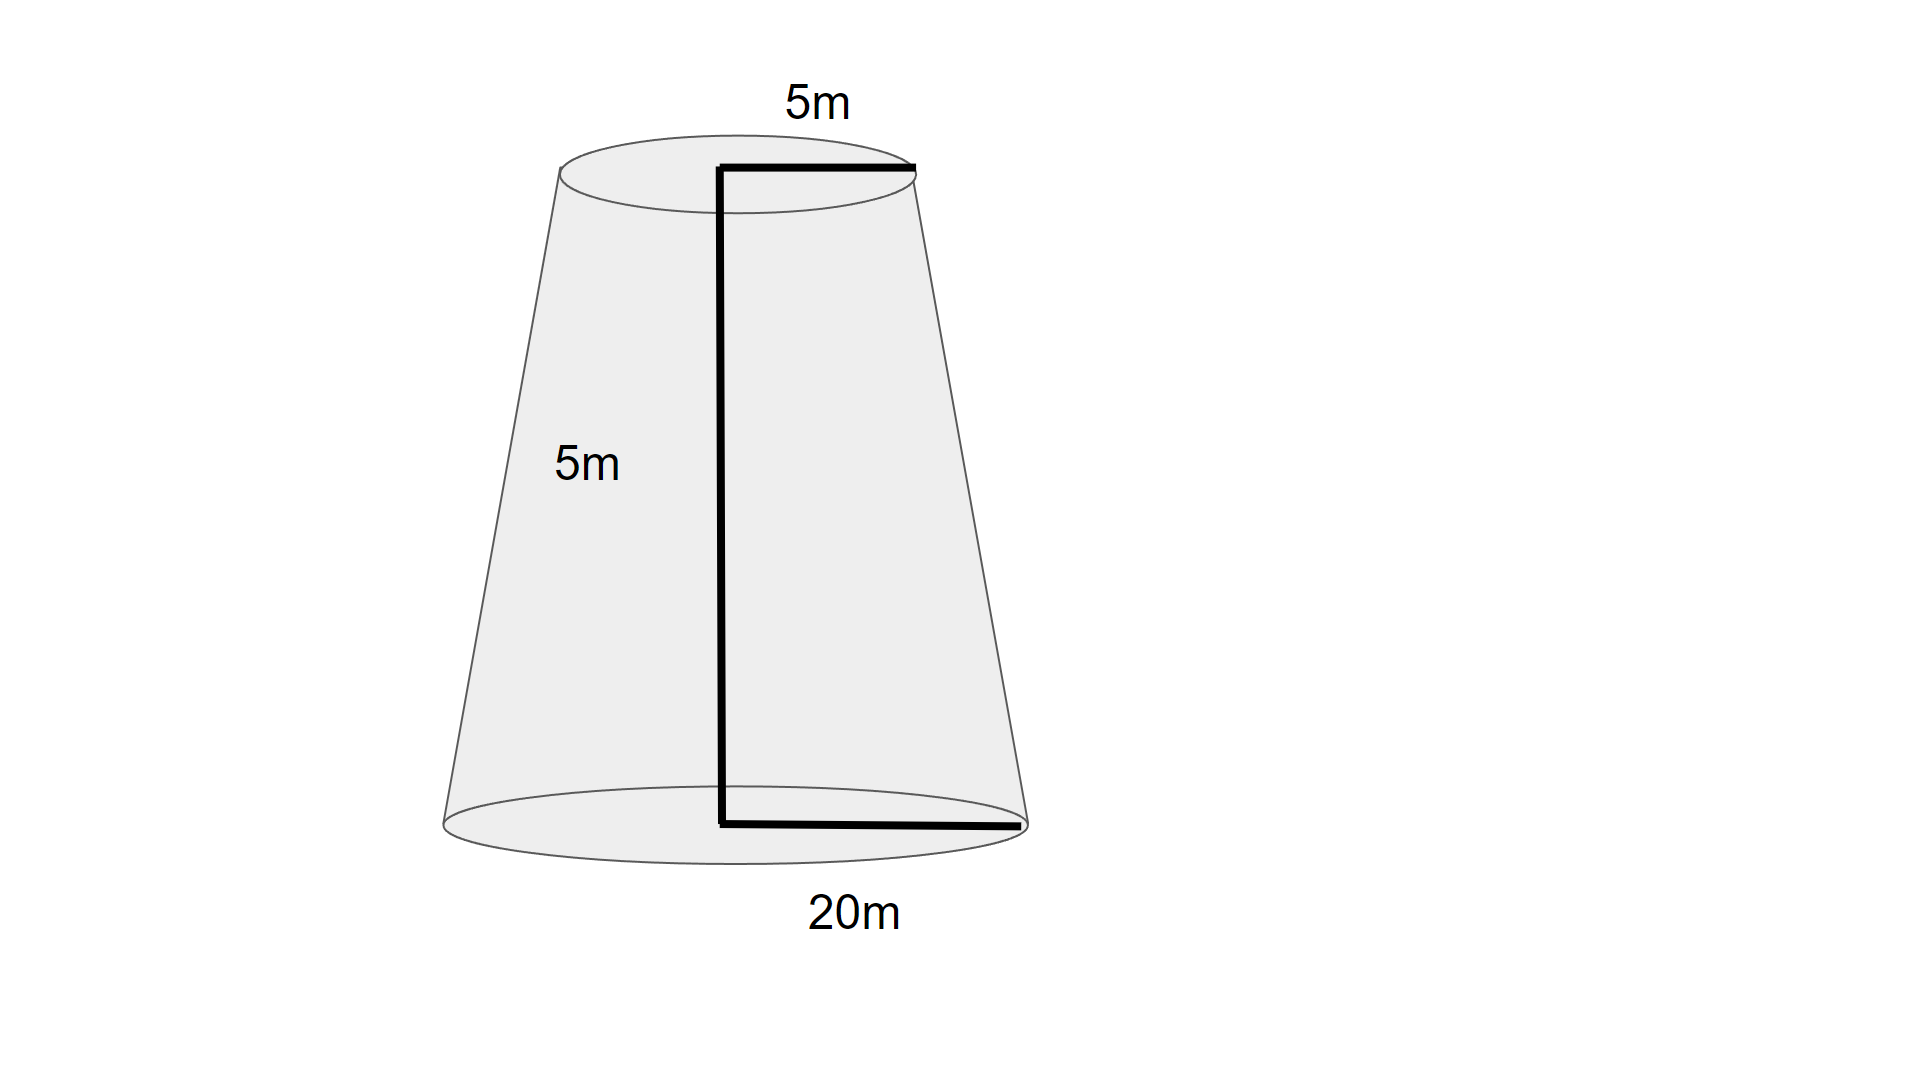
\includegraphics[width=10cm,scale=5]{img/回転体.png}
\end{figure}
\subsubsection*{解答}
この図を横にするとわかりやすいかもしれない。この図形の母線が$f(x)$である。
まずは$f(x)$を求めることにすると、$\displaystyle \frac{20-5}{5}=3$より、$f(x)=3x+5$
であることがわかる。よって体積は
\begin{equation*}
    \pi\int_0^5(3x+5)^2dx =\frac{\pi}{3}\int_5^{20} t^2dt=\frac{\pi}{3}\left[\frac{t^3}{3}\right]_5^{20}=\frac{\pi}{9}(20^3-5^3)=875\pi
\end{equation*}
\subsubsection*{例題}
半径$r$の球の体積を求めよ。
\subsubsection*{解答}
もちろん$V=\frac{4}{3}\pi r^3$であるのだが、ここでは積分を使って求めてみよう。$f(x)=\sqrt{r^2-x^2}$であるから
\begin{equation*}
    V=\pi\int_{-r}^{r}(\sqrt{r^2-x^2})^2dx=\pi\left[r^2x -\frac{x^3}{3}\right]_{-r}^r
    =2\pi\left(r^3-\frac{r^3}{3}\right)=\frac{4}{3}\pi r^3
\end{equation*}
これは、球の体積の公式の証明でもある。
\subsection{曲線の長さ}
次に、曲線の長さを積分で求める方法を考える。区間$a\leq x\leq b$の$y=f(x)$の長さ$L$は、
\begin{equation*}
    L=\int_a^b \sqrt{1+\left(\frac{dy}{dx}\right)^2}dx
\end{equation*}
で求められる。なぜならば、微小の長さ$dL$は、$\sqrt{dx^2+dy^2}$で表すことができるため、
これを変形して、$dL=\sqrt{1+\left(\frac{dy}{dx}\right)^2}dx$とし、この$a$から$b$までの積分が
$L$であるためである。
\subsubsection*{例題}
半径が$r$の円の円周を求めよ。
\subsubsection*{解答}
計算するまでもなく、$2\pi r$であるのだが、ここでは積分を使って答えを出そう。円周の長さを$l$とすると
\begin{equation*}
    \frac{l}{2}=\int_{-r}^r \sqrt{1+\left(-\frac{x}{\sqrt{r^2-x^2}}\right)^2}dx=r\int_{-r}^r \frac{dx}{\sqrt{r^2-x^2}}=\pi r
\end{equation*}
よって、$l=2\pi r$となる。
\subsubsection*{例題}
次の曲線の長さを求めよ。ただし、区間は$0$から$\pi$とする。
\begin{equation*}
    (1)y=\sqrt{3}x\quad (2)y=x^2 \quad(3)y=\cosh x
\end{equation*}
\subsubsection*{解答}
(1)普通に計算して、
\begin{equation*}
    \int_0^\pi \sqrt{1+(\sqrt{3})^2}dx=2\pi
\end{equation*}
もしくは、三平方の定理によって$\pi \cdot 2=2\pi$としてもよい。このように三平方の定理の一般化
として積分をとらえることもできる。

(2)こちらも公式を適応して、
\begin{equation*}
    \int_0^\pi \sqrt{1+(2x)^2}dx=\frac{1}{2}\int_0^{2\pi} \sqrt{1+x^2}dx =\frac{1}{4}\left(2\pi\sqrt{4\pi^2+1}+\log(2\pi+\sqrt{4\pi^2+1})\right)
\end{equation*}
となる。

(3)$(\cosh x)'=\sinh x$であるから、
\begin{equation*}
    \int_0^\pi \sqrt{1+\sinh^2 x}dx=\int_0^\pi \cosh xdx=\sinh\pi -\sinh 0=\sinh \pi
\end{equation*}
となる。
\newpage
\subsection{演習問題}
1.楕円$\displaystyle \frac{x^2}{a^2}+\frac{y^2}{b^2}=1$の面積を求めよ。\\

2.円錐の体積を$V$、高さを$h$、表面積を$S$とするとき、
\begin{equation*}
    V=\frac{1}{3}Sh
\end{equation*}
であることを証明せよ。\\

3.三平方の定理$a^2+b^2=c^2$を積分を用いて証明せよ。\\
\hrulefill
\subsection{$\blacksquare$CoffeeBreak:球の表面積}
\begin{screen}
    球の体積は積分で求められた。では、球の表面積はどのように求めればよいだろうか。結論から言うと、
    体積$\displaystyle V=\frac{4}{3}\pi r^3$を$r$で微分すればよい。実際に微分してみると、$V'=4\pi r^2$
    と確かに中学校で習った公式と一致する。この理由について考えてみる。まず、半径$x$の球の表面積を$S(x)$とする。
    さらに球の中心から$x+\Delta x$の球をつくる。このとき、$\Delta x$が十分に小さいとすると、外側の球の体積は
    $S(x)\Delta x$となる。この体積を$0$から$r$まで寄せ集めたのが、半径$r$の円の体積である。よって$\Delta x\to 0$とすると
    \begin{equation*}
        \int_0^r S(x)dx=\frac{4}{3}\pi r^3
    \end{equation*}
    両辺を$r$で微分すると
    \begin{equation*}
        \frac{d}{dr}\int_0^r S(x)dx=4\pi r^2
    \end{equation*}
    左辺は微積分学の基本定理より$S(r)$となるため、$S(r)=4\pi r^2$となる。\\\\

    ちなみに、一般的に回転体の表面積は次のように求まる。
    \begin{equation*}
        S=\int_a^b y\sqrt{1+\left(\frac{dy}{dx}\right)^2}dx
    \end{equation*}
    この公式に代入してみても、球の表面積は求まる。
\end{screen}
\newpage
\section{広義積分}
ここでは広義積分について扱っていく。広義積分は、積分区間に不連続点がある場合、もしくは区間の上限や下限が無限大である場合の積分であった。
関数$f(x)$でただ一つの不連続点$a\leq c\leq b$となる$c$がある場合、
\begin{equation*}
    \int_a^b f(x)dx=\lim_{\epsilon_1\to 0}\int_a^{c-\epsilon_1}f(x)dx+\lim_{\epsilon_2\to 0}\int_{\epsilon_2+c}^b f(x)dx
\end{equation*}
の右辺の極限が存在する場合は、広義積分は収束するといい、その極限値が広義積分の値となる。積分区間の上限が無限大の場合は、
\begin{equation*}
    \int_a^\infty f(x)dx=\lim_{b\to\infty}\int_a^b f(x)dx
\end{equation*}
脳編の極限値として、積分を定義する。もちろん、下限もしくは両方が無限の場合も同様である。
\subsection{広義積分の基礎}
始めに、簡単な広義積分の問題を解いてみよう。
\subsubsection*{例題}
以下の積分を求めよ。
\begin{equation*}
    (1)\int_0^1\frac{dx}{\sqrt{x}}\qquad(2)\int_0^\frac{\pi}{2} \frac{\cos x}{\sqrt{1-\sin x}}dx\qquad (3)\int_{-\infty}^\infty \frac{dx}{e^x+e^{-x}}
\end{equation*}
\subsubsection*{解答}
(1)$x=0$で特異的であるため、広義積分となる。
\begin{equation*}
    \int_0^1\frac{dx}{\sqrt{x}}=\lim_{\epsilon\to 0}\int_{\epsilon}^1\frac{dx}{\sqrt{x}}=\lim_{\epsilon\to 0}\left[2\sqrt{x}\right]_\epsilon^1=\lim_{\epsilon\to 0}2(1-\sqrt{\epsilon})=2
\end{equation*}
このように毎回極限の操作を表記するのは面倒なので、
\begin{equation*}
    \int_0^1\frac{dx}{\sqrt{x}}=\left[2\sqrt{x}\right]=2-0=2
\end{equation*}
という風に表記してもよい。\\

(2)$x=\frac{\pi}{2}$で特異的である。
\begin{equation*}
    \int_0^\frac{\pi}{2}\frac{\cos x}{\sqrt{1-\sin x}}dx=\int_{-1}^0 \frac{dt}{\sqrt{t+1}}dt=\left[2\sqrt{t+1}\right]_{-1}^0=2
\end{equation*}
となる。\\

(3)無限区間の積分である。
\begin{equation*}
    \int_{-\infty}^\infty \frac{dx}{e^x+e^{-x}}=\int_{-\infty}^\infty \frac{e^x}{e^{2x}+1}dx=\int_0^\infty \frac{dt}{t^2+1}=\frac{\pi}{2}
\end{equation*}
とよく知られた積分に帰着する。
\newpage
\subsubsection*{例題}
次の積分を求めよ。
\begin{equation*}
    G=\int_{-\infty}^{\infty}e^{-x^2}dx
\end{equation*}
\subsubsection*{解答}
こちらは有名なガウス積分である。多重積分を用いなくても求めることはできるが、随分と技巧的になってしまうので、今回は
多重積分を用いて自然に解く。いったん問題の積分を解く前に、次の積分を求める。
\begin{equation*}
    I=\int_{-\infty}^{\infty}\int_{-\infty}^{\infty}e^{-(x^2+y^2)}dy dx
\end{equation*}
極座標変換$(x,y)\to(r,\theta)$を行うことで、$x=r\cos\theta,y=r\sin\theta$となり、ヤコビアン$J$は
\begin{equation*}
    J=\begin{pmatrix}
        \displaystyle \frac{\partial x}{\partial r} & \displaystyle \frac{\partial x}{\partial \theta} \\\\
        \displaystyle \frac{\partial y}{\partial r} & \displaystyle \frac{\partial y}{\partial \theta}
     \end{pmatrix}
    =\cos\theta\cdot r\cos\theta + r\sin\theta\cdot\sin\theta =r
\end{equation*}
となる。よって、
\begin{equation*}
    I=\int_0^\infty dr\int_0^{2\pi}re^{-r^2}d\theta
\end{equation*}
と変形できるため、
\begin{equation*}
    I=2\pi\int_0^\infty re^{-r^2}dr=\pi 
\end{equation*}
と求まる。また、
\begin{equation*}
    I=\int_{-\infty}^{\infty}\int_{-\infty}^{\infty}e^{-(x^2+y^2)}dy dx=\int_{-\infty}^\infty e^{-x^2}dx\cdot\int_{-\infty}^\infty e^{-y^2}dy=\left(\int_{-\infty}^{\infty}e^{-x^2}dx\right)^2=G^2
\end{equation*}
であるため、
\begin{equation*}
    G^2=\pi
\end{equation*}
よって、$G=\sqrt{\pi}$となる。\\

もしくは次のようにしてもよい。$x\to\sqrt{t}x$の置換を行い、
\begin{equation*}
    \int_{-\infty}^{\infty}e^{-tx^2}dx=\frac{G}{\sqrt{t}}
\end{equation*}
とできることに注意する。また、
\begin{equation*}
    \int_0^{\infty}e^{-ax}dx=\frac{1}{a}
\end{equation*}
であることから、
\begin{equation*}
    \pi=\int_{-\infty}^{\infty}\frac{dx}{x^2+1}=\int_{-\infty}^{\infty}dx\int_0^{\infty}e^{-(x^2+1)t}dt=
    \int_{0}^{\infty}e^{-t}dt\int_{-\infty}^{\infty}e^{-x^2}dx=G\int_{0}^\infty\frac{e^{-t}}{\sqrt{t}}dt=G^2
\end{equation*}
よって、$G=\sqrt{\pi}$と求まる。こちらのやり方はヤコビアンを用いない分初歩的である。
\newpage
\subsection{収束因子}
広義積分を解くあたって、そのままでは収束しそうにないときに、パラメータ$\varepsilon$を導入して、収束値を求めたあとに
$\varepsilon\to 0$極限をとって収束値とするやり方がある。これを収束因子という。
\subsubsection*{例題}
\begin{equation*}
    \int_0^\infty \frac{\sin x}{x}dx
\end{equation*}
を求めよ。
\subsubsection*{解答}
収束因子を用いる。$\varepsilon,a>0$として、
\begin{equation*}
    I(\varepsilon)=\int_0^\infty e^{-\varepsilon x}\frac{\sin ax}{x}dx
\end{equation*}
を考える。$\mbox{Im}$は虚部を取ることとすると、
\begin{align*}
    I'(\varepsilon)&=-\mbox{Im}\left(\int_0^\infty e^{-x(\varepsilon-ai)}dx\right)=-\mbox{Im}\left(\frac{1}{\varepsilon-ai}\right)\\
    &=-\frac{a}{\varepsilon^2+a^2}
\end{align*}
よって、両辺を$\varepsilon$で積分してあげると
\begin{equation*}
    I(\varepsilon)=-\arctan\left(\frac{\varepsilon}{a}\right)+C
\end{equation*}
しかし、$I(\infty)=0$であるため、$C=\frac{\pi}{2}$でなければならない。
よって、
\begin{equation*}
    I(\varepsilon)=\frac{\pi}{2}-\arctan\left(\frac{\varepsilon}{a}\right)
\end{equation*}
ここで、$a=1,\varepsilon\to+0$の極限を取ると、$\displaystyle I(0)=\frac{\pi}{2}$となる。
少し技巧的にはなってしまったが、答えが求められたので良しとしよう。
\subsubsection*{例題}
\begin{equation*}
    I=\int_{-\infty}^\infty \sin(x^2)dx=\int_{-\infty}^\infty \cos(x^2)dx
\end{equation*}
を求めよ。
\subsubsection*{解答}
そのままだと計算が難しそうなので収束因子を用いる。
\begin{equation*}
    J(\varepsilon)=\int_{-\infty}^{\infty}e^{-x^2\varepsilon}\sin(x^2)dx=\mbox{Im}\left(\int_{-\infty}^{\infty}e^{-x^2(\varepsilon-i)}dx\right)
\end{equation*}
ここで、$\sqrt{\varepsilon-i}x\to x$の置換を施すと、$\mbox{Im}(\sqrt{\varepsilon-i})>0$であれば、ガウス積分に帰着するので、
\begin{equation*}
    =\mbox{Im}\left(\frac{1}{\sqrt{\varepsilon-i}}\int_{-\infty}^{\infty}e^{-x^2}dx\right)=\frac{\sqrt{\pi}}{\varepsilon^2+1}\mbox{Im}\left(\sqrt{\varepsilon-i}\right)
\end{equation*}
ここで極限$\varepsilon\to 0$を施すと、$\mbox{Im}(\sqrt{\varepsilon-i})$は、
\begin{equation*}
    \mbox{Im}(\sqrt{\varepsilon-i})=\mbox{Im}(i^{\frac{3}{2}})
\end{equation*}
さて、$\displaystyle e^{i\frac{\pi}{2}}=i$であるため、$i^{\frac{3}{2}}=e^{i\frac{3\pi}{4}}=-\frac{1}{\sqrt{2}}+\frac{i}{\sqrt{2}}$となる。虚部を取ると、
$Im(i^{\frac{3}{2}})=\frac{1}{\sqrt{2}}>0$となる。よって、ガウス積分に帰着しても大丈夫であることがわかる。積分の計算に話を戻すと、
\begin{equation*}
    J(0)=I=\sqrt{\frac{\pi}{2}}
\end{equation*}
となることがわかる。よって答えは、$\displaystyle I=\sqrt{\frac{\pi}{2}}$である。\\

もしくは別解として、置換$x^2=t$を行うと、
\begin{equation*}
    \int_{-\infty}^\infty \sin(x^2)dx=\int_{0}^{\infty}\frac{\sin(t)}{\sqrt{t}}dt
\end{equation*}
となる。ここで、
\begin{equation*}
    \frac{1}{\sqrt{t}}=\frac{1}{\sqrt{\pi}}\int_{-\infty}^{\infty}e^{-tx^2}dx
\end{equation*}
であることを思い出すと、
\begin{equation*}
    I=\frac{1}{\sqrt{\pi}}\int_{-\infty}^{\infty}dx\int_{0}^{\infty}e^{-tx^2}\sin(t)dt=\frac{1}{\sqrt{\pi}}\int_{-\infty}^{\infty}\frac{dx}{x^4+1}
\end{equation*}
最後の積分は演習問題でやることにしてここでは答えだけを書くと、
\begin{equation*}
    \int_{-\infty}^{\infty}\frac{dx}{x^4+1}=\frac{\pi}{\sqrt{2}}
\end{equation*}
であるため、結局答えは
\begin{equation*}
    I=\sqrt{\frac{\pi}{2}}
\end{equation*}
となる。この積分は、\textbf{フレネル積分}という。\\
\hrulefill\\
始めの例題の積分はフーリエ変換で解くのが一般的である。今回の例題の解き方は少々``技巧的すぎる''が、逆に言えば、
それでも高度な知識を用いずに解くことができるのを知ってほしい。同じような問題で、$\displaystyle \int_0^\infty dx\frac{\cos(ax)}{1+x^2}$
を少し技巧的に解くこともできる。普通は、フーリエの積分公式をつかってとく。ちなみにこの積分から、最初の積分を
導くこともできる。
\newpage
\subsection{その他の難しい広義積分}
最後に少し難しめの積分を解いていく。たくさん練習していこう。
\subsubsection*{例題}
\begin{equation*}
    (1)\int_0^\infty \frac{dx}{x^3+1}\qquad(2)\int_0^1\frac{\log(1+x)}{1+x^2}dx
\end{equation*}
\subsubsection*{解答}
(1)部分分数分解を行うと、
\begin{equation*}
    \frac{1}{x^3+1}=\frac{1}{(x+1)(x^2-x+1)}=\frac{1}{3}\left(\frac{1}{x+1}+\frac{-x+2}{x^2-x+1}\right)
\end{equation*}
よって積分は、
\begin{equation*}
    \frac{1}{3}\left(\int_0^\infty\frac{dx}{x+1}-\int_0^\infty \frac{x}{x^2-x+1}+2\int_0^\infty\frac{dx}{x^2-x+1}\right)
\end{equation*}
と変形する。一番左の積分は今のままでは発散してしまうので、真ん中と一番右の積分を計算する。真ん中の積分を$I$、一番右の積分を$J$として
計算を進める。先に$J$から計算する。
\begin{equation*}
    J=2\int_0^\infty \frac{dx}{x^2-x+1}=2\int_0^\infty \frac{dx}{(x-\frac{1}{2})^2+\frac{3}{4}}=\frac{4}{\sqrt{3}}\left[\arctan(\frac{x-\frac{1}{2}}{\sqrt{\frac{3}{4}}})\right]_0^\infty =\frac{8\pi}{3\sqrt{3}}
\end{equation*}
と簡単に求まる。次に$I$を計算する。$x-\frac{1}{2}=t$の置換を行うと、積分は  
\begin{equation*}
    I=\int_{-\frac{1}{2}}^\infty \frac{t}{t^2+\frac{3}{4}}dt+\frac{1}{2}\int_{-\frac{1}{2}}^\infty \frac{dt}{t^2+\frac{3}{4}} 
\end{equation*}
の二つに分けられる。右の積分は、$\displaystyle\frac{2\pi}{3\sqrt{3}}$となるので、左の積分を計算すると
\begin{equation*}
    \int_{-\frac{1}{2}}^{\infty}\frac{t}{t^2+\frac{3}{4}}dt=\frac{1}{2}\left[\log(t^2+\frac{3}{4})\right]_{-\frac{1}{2}}^\infty
\end{equation*}
となり、発散してしまう。ここでいったん今までの積分をまとめると、
\begin{equation*}
    \frac{1}{3}\left(\left[\log(x+1)\right]_0^\infty -\frac{1}{2}\left[\log(t^2+\frac{3}{4})\right]_{-\frac{1}{2}}^\infty+\frac{2\pi}{\sqrt{3}}\right)
\end{equation*}
真ん中の項の変数を、$x$に戻してあげると一つ目の項とまとめることができるので
\begin{equation*}
    \left[\log(x+1)-\frac{1}{2}\log((x-\frac{1}{2})^2+\frac{3}{4})\right]_0^\infty=\lim_{a\to\infty}\frac{1}{2}\log\left(\frac{(a+1)^2}{(a-\frac{1}{2})^2+\frac{3}{4}}\right)
\end{equation*}
となり、ド・ロピタルの定理によって真数は$1$となるため、極限値は$0$となる。よって最終的には
\begin{equation*}
    \int_0^\infty\frac{dx}{x^3+1}=\frac{2\pi}{3\sqrt{3}}
\end{equation*}

ここの計算で特に面倒だったのが$J$以外の計算である。部分分数分解も計算が大変であった。この計算を避ける方法として、
別解がある。まず、積分を$I$としておき、$x\to\frac{1}{x}$の置換を行う。すると、
\begin{equation*}
    I=\int_\infty^0\frac{-\frac{1}{x^2}}{(\frac{1}{x})^3+1}dx=\int_0^\infty \frac{x}{x^3+1}dx
\end{equation*}
と変形できるため、最初の積分と足して
\begin{equation*}
    I=\frac{1}{2}\int_0^\infty \frac{x+1}{x^3+1}dx=\frac{1}{2}\int_0^\infty \frac{x+1}{(x+1)(x^2-x+1)}dx=\frac{1}{2}\int_0^\infty\frac{dx}{x^2-x+1}=\frac{2\pi}{3\sqrt{3}}
\end{equation*}
と、はるかに簡単に求まる。

(2)$x=\tan\theta$で置換する。
\begin{equation*}
    I=\int_0^\frac{\pi}{4}\frac{\log(1+\tan\theta)}{\frac{1}{\cos^2\theta}}\frac{1}{\cos\theta}d\theta=\int_0^\frac{\pi}{4}\log(1+\tan\theta)d\theta
\end{equation*}
ここで
\begin{equation*}
    \log(1+\tan\theta)=\log\left(\frac{1}{\cos\theta}(\cos\theta+\sin\theta)\right)=-\log(\cos\theta)+\log(\sqrt{2}\sin(\theta+\frac{\pi}{4}))=-\log(\cos\theta)+\log(\sin(\theta+\frac{\pi}{4}))+\frac{1}{2}\log(2)
\end{equation*}
と変形できるので、
\begin{equation*}
    \frac{1}{2}\log 2\int_0^\frac{\pi}{4}d\theta +\int_0^\frac{\pi}{4}\log(\sin(\theta+\frac{\pi}{4}))d\theta-\int_0^\frac{\pi}{4}\log(\cos\theta)d\theta
\end{equation*}
さらに、真ん中の積分は$\theta\to\frac{\pi}{4}-\theta$の置換によって、
\begin{equation*}
    \int_0^\frac{\pi}{4}\log(\sin(\theta+\frac{\pi}{4}))d\theta=\int_0^\frac{\pi}{4}\log(\sin(\frac{\pi}{2}-\theta))d\theta=\int_0^\frac{\pi}{4}\log(\cos\theta)d\theta
\end{equation*}
となり、第三項と打ち消しあうので、
\begin{equation*}
    I=\frac{1}{2}\log 2\int_0^\frac{\pi}{4}d\theta=\frac{\pi\log 2}{8}
\end{equation*}
となる。
\subsubsection*{例題}
次の積分を求めよ。
\begin{equation*}
    (1)\int_a^b\frac{dx}{\sqrt{(x-a)(b-x)}}\qquad(2)\int_a^b\frac{dx}{x\sqrt{(x-a)(b-x)}}
\end{equation*}
ただし、どちらも$b>a>0$とする。
\subsubsection*{解答}
(1)見た目からも$1/\sqrt{1-x^2}$の積分に帰着させることがなんとなくわかるが、一応計算してみよう。
分母の平方根の中は、
\begin{equation*}
    (x-a)(b-x)=-x^2+(a+b)x-ab=-\left(x-\frac{a+b}{2}\right)^2+\frac{a^2+b^2+2ab}{4}-\frac{4ab}{4}
    =-\left(x-\frac{a+b}{2}\right)^2+\left(\frac{b-a}{2}\right)^2
\end{equation*}
と変形できる。よって、$A=\frac{b-a}{2}$、$x-\frac{a+b}{2}=t$と置換すると、
\begin{equation*}
    \int_{-A}^{A}\frac{dt}{\sqrt{A^2-t^2}}=\left[\arcsin\left(\frac{t}{A}\right)\right]_{-A}^A=\pi
\end{equation*}
となる。
\newpage
別解として、置換$x=a\cos^2\theta+b\sin^2\theta$とすると、$dx=2(b-a)\sin\theta\cos\theta d\theta$となるため
\begin{equation*}
    2(b-a)\int_{0}^{\frac{\pi}{2}}\frac{\sin\theta\cos\theta}{\sqrt{(b-a)^2\sin^2\theta\cos^2\theta}}d\theta=2\int_0^\frac{\pi}{2}d\theta=\pi
\end{equation*}
となる。\\

(2) 1の別解と同じ置換を用いると、
\begin{equation*}
    2\int_0^\frac{\pi}{2}\frac{d\theta}{a\cos^2\theta+b\sin^2\theta}
\end{equation*}
と変形できるので、これを解くと、
\begin{equation*}
    =2\left[\frac{1}{\sqrt{ab}}\arctan\left(\sqrt{\frac{b}{a}}\tan\theta\right)\right]_0^\frac{\pi}{2}=\frac{\pi}{\sqrt{ab}}
\end{equation*}
となる。
\subsubsection*{例題}
次の積分を求めよ。
\begin{equation*}
    (1)\int_0^\frac{\pi}{2}\log(\cos x)dx\qquad(2)\int_0^1 \log\frac{x}{(1-x)^2}dx\qquad(3)\int_{-\infty}^{\infty}\frac{dx}{ax^2+bx+c}\quad(a>0,b^2-4ac<0)
\end{equation*}
\subsubsection*{解答}
これがこの章最後の例題である。

(1)まずは、$x\to\frac{\pi}{2}-x$の置換によって、
\begin{equation*}
    I=\int_0^\frac{\pi}{2}\log(\cos x)dx=\int_0^\frac{\pi}{2}\log(\sin x)dx
\end{equation*}
であることがわかる。よって、対数の性質$\log x+\log y=\log(xy)$より、
\begin{equation*}
    I=\frac{1}{2}\int_0^\frac{\pi}{2}\log(\sin x\cos x)dx=\frac{1}{2}\int_0^\frac{\pi}{2}\log(\frac{1}{2}\sin(2x))dx
\end{equation*}
さらに、$2x\to x$より、
\begin{equation*}
    I=\frac{1}{4}\int_0^\pi \log(\frac{1}{2}\sin x)dx=-\frac{\pi}{4}\log 2+\frac{1}{2}I
\end{equation*}
であるため、移項して
\begin{equation*}
    I=-\frac{\pi}{2}\log 2
\end{equation*}
となる。\\

(2)式を簡単にして、
\begin{equation*}
    I=\int_0^1 \log x -2\log(1-x)dx=\int_0^1 \log x dx -2\int_0^1 \log(1-x)dx=-\int_0^1\log xdx
    =-\left[x\log x- x\right]_0^1=1
\end{equation*}
途中の積分は、$1-x\to x$でまとめることができる。
\newpage
(3)条件から、分母の二次式は常に正であることがわかる。問題には正直何の関係もないのだが一応確認のために書いておいた。
さて、問題の積分だが、いつも通り平方完成してみよう。
\begin{equation*}
    I=\int_{-\infty}^{\infty}\frac{dx}{ax^2+bx+c}=\frac{1}{a}\int_{-\infty}^{\infty}\frac{dx}{x^2+\frac{b}{a}x+\frac{c}{a}}=\frac{1}{a}\int_{-\infty}^{\infty}\frac{dx}{(x+\frac{b}{2a})^2+\frac{4ac-b^2}{4a^2}}
\end{equation*}
条件より、$\displaystyle\frac{4ac-b^2}{4a^2}>0$であるため、$\displaystyle \int\frac{dx}{1+x^2}$の積分として解ける。よって、
\begin{equation*}
    I=\frac{2}{\sqrt{4ac-b^2}}\left[\arctan\left(\frac{x+\frac{b}{2a}}{\sqrt{\frac{4ac-b^2}{4a^2}}}\right)\right]_{-\infty}^\infty=\frac{2\pi}{\sqrt{4ac-b^2}}
\end{equation*}
となる。
\newpage
\subsection{演習問題}
次の積分を解け。\\\\
(1)$\displaystyle \int_0^\infty \frac{x^2}{(1+x^2)^2}dx$
\hspace{15mm}
(2)$\displaystyle \int_0^\infty \left(\frac{\sin x}{x}\right)^2 dx$
\hspace{15mm}
(3)$\displaystyle \int_0^\infty \frac{dx}{1+x^4}$
\hspace{15mm}
(4)$\displaystyle \int_0^\infty \frac{\log x}{1+x^2}dx$
\\\\
(5)$\displaystyle \int_0^a \frac{x}{\sqrt{ax-x^2}}dx\quad(a>0)$
\\

平均$\mu$、分散$\sigma^2$の正規分布の確率密度関数$\displaystyle f(x)=\frac{e^{\frac{-(x-\mu)^2}{2\sigma^2}}}{\sqrt{2\pi\sigma^2}}$ は規格化されている(=確率の総和は1)。これを示せ。
なお、これを積分で表すと、
\begin{equation*}
    \int_{-\infty}^{\infty}f(x)dx
\end{equation*}
となる。\\
\hrulefill
\subsection{$\blacksquare$CoffeeBreak:オイラーの等式を用いて積分を簡単に}
\begin{screen}
    すでに何回か登場しているが、オイラーの等式を用いることで積分を簡単に表すことができる場合がある。
    たとえば、「収束因子」の章の例題などがそれにあたる。三角関数と指数関数$e^x$の積を$e^{x}$の形で表せると、
    微分積分が簡単になるのはすでに体験しているだろう。これらは本来は複素関数の範囲なのだが、実数の場合同様に
    微分積分できるためこれが成り立つ。詳しくは複素関数で学べるだろう。話を戻すが、このやり方は別に広義積分以外
    でも使うことができる。たとえば、
    \begin{equation*}
        \int e^{ax} \cos bx dx
    \end{equation*}
    をオイラーの等式を用いて計算してみよ。答えが同じになるはずである。
\end{screen}
\newpage
\part{補足}
ここでは特殊な関数や積分を紹介したりする。よく表れて役に立つものばかりである。
\section{ガンマ関数$\Gamma(s)$}
ガンマ関数$\Gamma(s)$は、
\begin{equation*}
    \Gamma(s)=\int_0^\infty x^{s-1}e^{-x}dx
\end{equation*}
のように定義される。$Re(s)>0$となる数に対して定義されるため、ガンマ関数は複素数でも定義される。
しかし今回は、$s\in \mathbb{R}>0$に限るとする。ガンマ関数には様々な性質がある。例題で一緒に見ていこう。
\subsubsection*{例題}
次の性質を証明せよ。
\begin{equation*}
    1.\Gamma(s+1)=s\Gamma(s)\qquad 2.\Gamma(1)=1\qquad 3.\Gamma(\frac{1}{2})=\sqrt{\pi}
\end{equation*}
\subsubsection*{解答}
1.
\begin{equation*}
\Gamma(s+1)=\int_0^\infty x^s e^{-x}dx =\left[-x^s e^{-x}\right]_0^\infty+s\int_0^\infty x^{s-1}e^{-x}dx=s\Gamma(s)  
\end{equation*}

2.
\begin{equation*}
    \Gamma(1)=\int_0^\infty e^{-x}dx=1
\end{equation*}

3.
\begin{equation*}
    \Gamma\left(\frac{1}{2}\right)=\int_0^\infty \frac{e^{-x}}{\sqrt{x}}dx=2\int_0^\infty e^{-x^2}dx=\sqrt{\pi}
\end{equation*}
\subsubsection*{}
これらの性質から、$n$が自然数のときは$\Gamma(n+1)=n!$が導ける。
\subsubsection*{例題}
\begin{equation*}
    \Gamma\left(\frac{4}{3}\right)=\int_0^\infty dx e^{-x^3}
\end{equation*}
を示せ。
\subsubsection*{解答}
\begin{equation*}
    \Gamma\left(\frac{4}{3}\right)=\frac{1}{3}\Gamma\left(\frac{1}{3}\right)=\frac{1}{3}\int_0^\infty \frac{e^{-x}}{\sqrt[3]{x^2}}
\end{equation*}
と変形できるので、$\sqrt[3]{x}\to x$と置換してあげると、$x\to x^3$であるため、
\begin{equation*}
    \Gamma\left(\frac{4}{3}\right)=\int_0^\infty e^{-x^3}dx
\end{equation*}
となり、示せた。
\section{ベータ関数$B(\alpha,\beta)$}
オイラーによって導入されたベータ関数は次のように定義される。
\begin{equation*}
    B(\alpha,\beta)=\int_0^1 x^{\alpha-1}(1-x)^{\beta-1}dx\quad(\alpha,\beta>0)
\end{equation*}
最後の条件は、積分の上限や下限の収束条件である。試しに$\beta=1$で$\alpha$に$0$や負の数を代入してみるとよい。
\subsubsection*{例題}
次の性質を証明せよ。
\begin{equation*}
    1.B(\alpha,\beta)=B(\beta,\alpha)\quad 2.B(\alpha,\beta)=\int_0^\infty \frac{x^{\alpha-1}}{(1+x)^{\alpha+\beta}}dx\qquad 3.\int_0^\frac{\pi}{2}\sin^m x\cos^n xdx=\frac{1}{2}B(\frac{m+1}{2},\frac{n+1}{2})\quad(m,n=0,1,...)
\end{equation*}
\subsubsection*{解答}
1.$1-x\to x$とすれば明らかである。
\begin{equation*}
    B(\alpha,\beta)=-\int_1^0 (1-x)^{\alpha-1}x^{\beta-1}dx=B(\beta,\alpha)
\end{equation*}\\

2.$\displaystyle x=\frac{t}{1+t}$と置換する。
\begin{equation*}
    B(\alpha,\beta)=\int_0^\infty \left(\frac{t}{1+t}\right)^{\alpha-1}\left(\frac{1}{1+t}\right)^{\beta-1}\frac{dt}{(1+t)^2}=\int_0^\infty \frac{t^{\alpha-1}}{(1+t)^{\alpha+\beta}}dt
\end{equation*}
普段はあまり行わない置換だったので難しかっただろう。\\

3.$t=\sin x$の置換を行うと、$t=\sqrt{1-\cos^2 x}$より、$\cos x=\sqrt{1-t^2}$、$dt=\cos x dx=\sqrt{1-t^2}dx$、
\begin{equation*}
    \int_0^\frac{\pi}{2}\sin^m x\cos^n xdx=\int_0^1 t^m(\sqrt{1-t^2})^n\frac{dt}{\sqrt{1-t^2}}=\int_0^1 t^m (1-t^2)^{\frac{n-1}{2}}dt
\end{equation*}
よって、$t^2=u$の置換を行えば、
\begin{equation*}
    =\frac{1}{2}\int_0^1t^{\frac{m-1}{2}}(1-m)^{\frac{n-1}{2}}dt=\frac{1}{2}\int_0^1t^{\frac{m+1}{2}-1}(1-m)^{\frac{n+1}{2}-1}dt=\frac{1}{2}B\left(\frac{m+1}{2},\frac{n+1}{2}\right)
\end{equation*}
となる。
\newpage
\subsubsection*{例題}
次の値を求めよ。
\begin{equation*}
    B\left(\frac{1}{2},s\right)=B\left(s,\frac{1}{2}\right)\quad(\text{ただし、}s=\frac{1}{2},1,\frac{3}{2},2,...)
\end{equation*}
\subsubsection*{解答}
これは、ウォリス積分を解くことと同義であることに気づけば、$\frac{n+1}{2}=s$より、$n=2s-1$。よって、
$s$が分数ならば、
\begin{equation*}
    B\left(\frac{1}{2},s\right)=\frac{(4s-3)!!}{(4s-2)!!}\frac{\pi}{2}
\end{equation*}
$s$が自然数ならば、
\begin{equation*}
    B\left(\frac{1}{2},s\right)=\frac{(4s-2)!!}{(4s-1)!!}
\end{equation*}
となる。
\section{ゼータ関数$\zeta(s)$}
次の級数$\zeta(s)$
\begin{equation*}
    \zeta(s)=\sum_{n=1}^\infty \frac{1}{n^s}\quad(s>1)
\end{equation*}
をリーマンのゼータ関数と呼ぶ。$s>1$は知っている通り、級数の収束条件である。ちなみに$s=2$とすると、
\begin{equation*}
    \zeta(2)=\frac{\pi^2}{6}
\end{equation*}
となる。
\section{完全楕円積分}
次の定積分を
\begin{equation*}
    K(k)=\int_0^\frac{\pi}{2}\frac{d\theta}{\sqrt{1-k^2\sin^2\theta}}\quad(0\leq k<1)\qquad E(k)=\int_0^\frac{\pi}{2}\sqrt{1-k^2\sin^2\theta}d\theta\quad(0\leq k\leq 1)
\end{equation*}
それぞれ第一種、第二種の完全楕円積分という。
\subsubsection*{例題}
\begin{equation*}
    K(0)=\frac{\pi}{2}\qquad E(0)=\frac{\pi}{2}\qquad E(1)=1
\end{equation*}
を示せ。
\subsubsection*{解答}
\begin{align*}
    K(0)&=\int_0^\frac{\pi}{2}d\theta=\frac{\pi}{2}\qquad E(0)=\int_0^\frac{\pi}{2}d\theta=\frac{\pi}{2}\\
    E(1)&=\int_0^\frac{\pi}{2}\sqrt{1-\sin^2\theta}d\theta=\int_0^\frac{\pi}{2}\cos\theta d\theta=1
\end{align*}
\hrulefill
\subsection*{$\blacksquare$CoffeeBreak:他分野との関連性}
\begin{screen}
    ここまで積分の計算のみに焦点をあてているので、他分野との関連性について軽く述べておく。
    真っ先に浮かぶのが物理だろう。有名な運動の法則$\displaystyle F=m\frac{d^2}{dt^2}x$で
    さえ、微分を使って書かれている。もちろんこの\textbf{微分方程式}を解くには、微積分、特に
    積分の知識が必要である。同じ積分つながりで線積分というものがある。物理の仕事は線積分を
    用いて計算できる。多重積分を用いれば、場所で異なる密度をもつ物体の質量なども求められる。
    ただ面積、体積が求められるだけではないのだ。\\
    物理以外にも、多くの分野で微分積分が使われている。たいていの本も、微分積分をマスターして
    いることが基準になっている(と思う)。計算ができなくて躓かないようにこの資料に書いてある
    計算はある程度マスターしておこう。
\end{screen}
\newpage
\part{確認問題}
最後の確認として解くのがいいと思う。簡単な積分から難しい積分まで集めている。\\
\hrulefill\\
1.次の積分を求めよ。\\

(1)$\displaystyle \int(x+1)(2-x)dx$
\hspace{10mm}
(2)$\displaystyle \int(x^2+a^2)^3dx$
\hspace{10mm}
(3)$\displaystyle \int\sin(\pi-x)dx$
\hspace{10mm}
(4)$\displaystyle \int (2e)^{x}dx$\\

(5)$\displaystyle \int(x+e)^e dx$
\hspace{19mm}
(6)$\displaystyle \int\frac{6x-1}{x^2-x-6}dx$
\hspace{9mm}
(7)$\displaystyle \int \frac{dx}{x^3+1}dx$
\hspace{15mm}
(8)$\displaystyle \int\frac{dx}{(x^2+a^2)^2}dx$\\

(9)$\displaystyle \int_1^2\log x dx$
\hspace{22mm}
(10)$\displaystyle \int\frac{\sqrt{x^2+1}}{x}dx$
\hspace{10mm}
(11)$\displaystyle \int_a^b(x-a)(b-a)dx$
\hspace{1mm}
(12)$\displaystyle \int\frac{dx}{\sinh x}$\\

2.次の積分を求めよ。\\

(1)$\displaystyle \int_0^\infty \frac{e^{-\sqrt{x}}}{\sqrt{x}}dx$
\hspace{17mm}
(2)$\displaystyle \int_0^1 \frac{x\log x}{(1+x)^4}dx$
\hspace{10mm}
(3)$\displaystyle \int_0^\frac{\pi}{4}\frac{x}{\sin 2x+2\cos^2 x}dx$
\hspace{10mm}
(4)$\displaystyle \int_0^\frac{\pi}{2} \left(\frac{\pi}{2}-x\right)\tan xdx$\\

(5)$\displaystyle \int_0^1\frac{\log x}{x^{a}}dx\hspace{1mm}(0<a<1)$
\hspace{0.5mm}
(6)$\displaystyle \int_{-1}^1 \frac{dx}{(1-2ax+a^2)\sqrt{1-x^2}}dx$\\

{\scriptsize ヒント:(6)は$x=\cos\theta$と置換せよ。}\\

3.次の積分を示せ。
\begin{equation*}
    \int_0^{2\pi}e^{inx}dx=\left \{
        \begin{array}{l}
            2\pi\quad(n=0)\\
            0 \quad\hspace{2mm}(n\neq 0)
        \end{array}
    \right.
\end{equation*}\\

4.次の(1)(2)に答えよ。

(1)次の積分を示せ。(ただし、$n=0,1,2,3...$)
\begin{equation*}
    I_n=\int_{n\pi}^{(n+1)\pi}dx e^{-x}\sin x=\frac{(-1)^n}{2}e^{-n\pi}(1+e^{-\pi})
\end{equation*}

(2)上の結果を用いて、次の積分を導出せよ。
\begin{equation*}
    I=\int_0^\infty dx e^{-x}|\sin x|=\frac{1}{2}\cdot \frac{1+e^{-\pi}}{1-e^{-\pi}}
\end{equation*}\\

5.($n=1,2,3,..$)として、次の積分を求めよ。
\begin{equation*}
    I_n=\int_{-\infty}^{\infty}\frac{dx}{(1+x^2)^{n+1}}
\end{equation*}\\

6.次の$x$軸を回転軸とする回転体の体積を求めよ。
\begin{figure}[h]
    \centering
    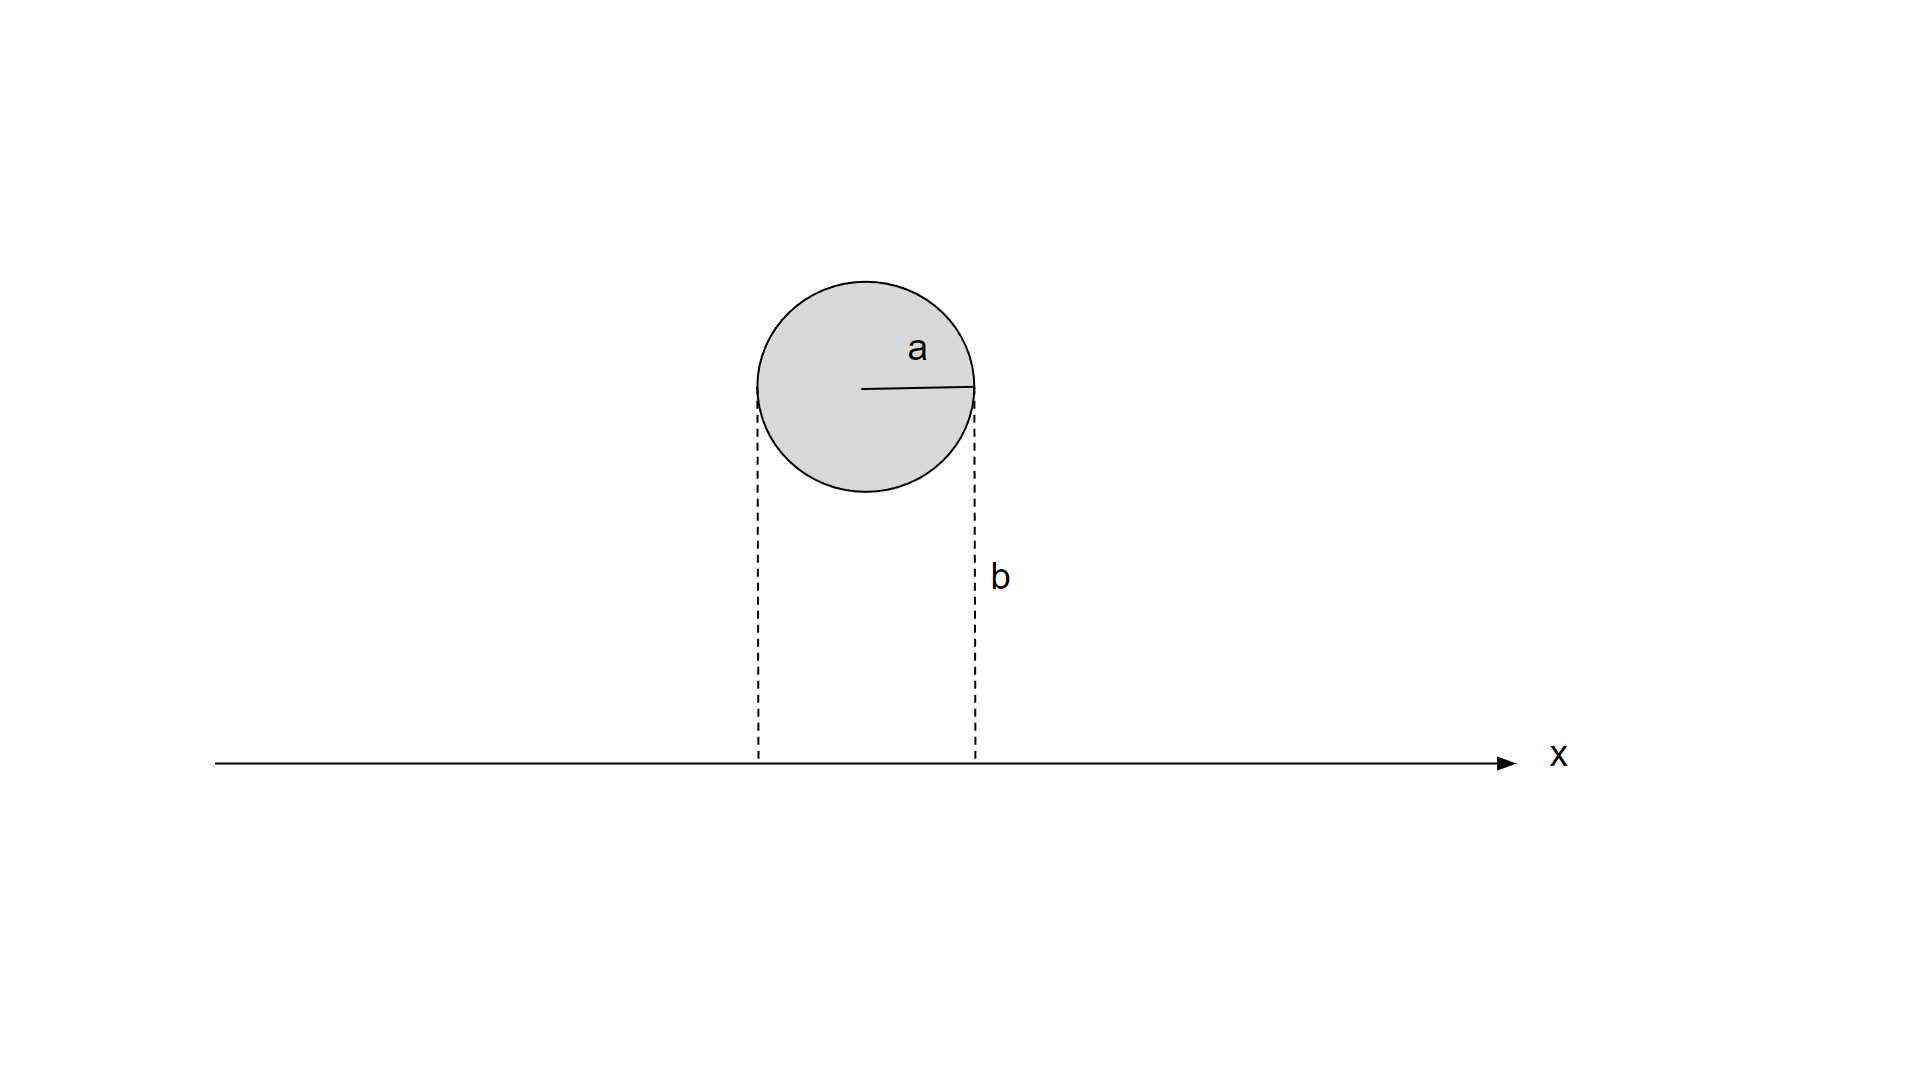
\includegraphics[width=15cm,scale=5]{img/回転体問題.png}
\end{figure}
このような図形を\textbf{トーラス体}という。\\

7.$n$を整数とすると、
\begin{equation*}
    \int x^{2n+1}\sqrt{x^2+1}dx
\end{equation*}
は必ず積分できる。これを示せ。\\

6.定積分
\begin{equation*}
    \int_0^\infty\frac{\cos(ax)}{1+x^2}=\frac{\pi}{2}e^{-|a|}
\end{equation*}
を次の手順で示せ。

(1)
\begin{equation*}
    \int_0^\infty \frac{\sin(ax)}{x}dx=\frac{\pi}{2}\mbox{sign}(a)    
\end{equation*}

(2)
\begin{equation*}
    \int_0^\infty \frac{\cos(ax)\sin(ax)}{x}dx=\frac{\pi}{4}\{\mbox{sign}(a+b)-\mbox{sign}(a-b)\}
\end{equation*}

(3)\hspace{2mm}(2)の両辺を$\displaystyle \int_0^\infty db\hspace{1mm}e^{-b}$して、求める定積分を導け。\footnote{この操作をラプラス変換という。記号で書くと、$\mathcal{L}[f(x)]$である。詳しくはフーリエ解析で学ぶ。}\\
\\
引用している問題のほうが多いので、ここまでの知識で解けるはずである。わからない問題はいったん飛ばして
次の問題に行くほうがいい。次の問題が前の問題のヒントになっているかもしれないからである。
\newpage
\part{解答}
以下解答である。
\\
\hrulefill\\

{\huge 随時更新予定}
\end{document}
